\documentclass{article}

\usepackage[preprint]{neurips_2025}

\usepackage[utf8]{inputenc}
\usepackage[T1]{fontenc}
\usepackage{hyperref}
\usepackage{url}
\usepackage{booktabs}
\usepackage{amsfonts}
\usepackage{nicefrac}
\usepackage{microtype}
\usepackage{xcolor}
\usepackage{graphicx}
\usepackage{float}
\usepackage{multirow}
\usepackage{subcaption}
% pdflatex -interaction=nonstopmode -halt-on-error report.tex
\title{Adaptive Atmospheric Turbulence Restoration for Remote Sensing Images with Generative Models}

\author{%
  Sitian Ding \\
  \texttt{2025011222} \\
  \And
  Jiamu Qin \\
  \texttt{2025011005} \\
  \And
  Wenyuan Huang \\
  \texttt{2025011051} \\
}

\begin{document}

\maketitle

\begin{abstract}
Atmospheric turbulence introduces spatially varying blur, geometric warping, and temporal instability that significantly degrade long-range remote sensing imagery. Unlike standard image corruption, turbulence is non-uniform across space and time, which makes direct restoration difficult and also makes paired real-world supervision scarce. In this project, we formulate adaptive atmospheric turbulence restoration for remote sensing as a supervised image-to-image translation problem driven by physically simulated degradations. We build a compact training pipeline on top of UC Merced Land Use and NWPU-RESISC45 imagery, synthesize turbulence-corrupted seven-frame sequences with a TurbulenceSim-based simulator, and train both a multi-frame U-Net baseline and a TSR-WGAN model. On the validation split, the best U-Net reaches 35.34 dB PSNR and 0.9804 SSIM, while TSR-WGAN reaches 34.14 dB PSNR and 0.9712 SSIM after training on mixed turbulence strengths. Qualitative results show improved recovery of roads, parking lots, buildings, and man-made boundaries under strong blur and local distortion. Code and assets are available at \url{https://github.com/Mars-Dingdang/DL-AdaptiveOptics}, and the dataset release is available at \url{https://huggingface.co/datasets/Mars-Dingdang/DL-AdaptiveOptics}.
\end{abstract}

\section{Introduction}
Atmospheric turbulence is a major challenge for long-range imaging, surveillance, astronomy, and remote sensing. Temperature and pressure fluctuations cause random variations in the refractive index along the optical path, which in turn induce geometric dancing, spatially varying blur, and local intensity fluctuations. In imagery, the most visible artifacts are wavy edges, unstable fine structures, and locally inconsistent sharpness. A recent review by Hill et al. emphasizes that turbulence is especially difficult because the distortion is spatially varying and spatio-temporal rather than globally shift-invariant or static \citep{hill2024review}. These effects reduce human interpretability and degrade downstream tasks such as scene classification, land-use analysis, and object recognition. 

\begin{figure}[H]
    \centering
    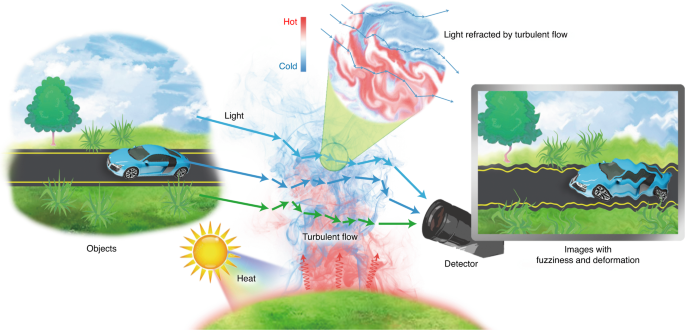
\includegraphics[width=0.6\linewidth]{images/atmosturbu.png}
    \caption{Schematic of imaging through atmospheric turbulence, extracted from \citet{{jin2021}}.}

\end{figure}

For remote sensing, the restoration problem is even harder than for common natural images. First, aerial and satellite scenes often contain repeated textures, man-made lines, and small semantic targets whose visibility depends on high-frequency spatial detail. Second, collecting paired data with both turbulence-corrupted observations and perfectly aligned clean ground truth is usually impractical. Third, turbulence in real imaging systems interacts with viewing distance, aperture, focal length, wavelength, wind speed, and scene depth, so synthetic approximations must balance fidelity and throughput.

Existing restoration methods fall into two broad families. Adaptive optics methods physically correct the distorted wavefront using specialized hardware, but they are expensive and not always practical for remote sensing acquisition pipelines. Image processing and learning-based methods instead aim to invert the corruption in software. Earlier classical approaches relied on registration, lucky-region fusion, deconvolution, or low-rank priors, while recent deep models learn the restoration mapping directly from data. TSR-WGAN showed that spatio-temporal generative modeling can recover complex scenes from turbulence sequences \citep{jin2021}. LTT-GAN further demonstrated that adversarial learning and latent inversion can restore images through turbulence more effectively than purely hand-crafted methods \citep{mei2023lttgan}. Diffusion-based restoration has recently become attractive because it can model highly multimodal inverse problems and incorporate physical priors or zero-shot constraints \citep{wang2023ddnm,jaiswal2023physics}.

However, most turbulence restoration literature targets surveillance or generic natural images. Remote sensing has different texture statistics, larger viewpoint variation, and stronger dependence on structural fidelity. This project therefore focuses on a practical remote sensing setting and asks a narrower question: can a relatively compact, physically grounded pipeline already provide strong turbulence restoration on remote sensing patches using limited training data? Our answer is to combine public aerial scene datasets with a TurbulenceSim-style degradation model and train a multi-frame U-Net that exploits temporal redundancy across seven turbulence-corrupted observations. In this formulation, the task becomes learning a mapping from a degraded sequence to a clean reference image, which preserves the physical motivation of adaptive optics while remaining tractable as a deep learning course project.

\section{Method}
Our pipeline consists of three stages: selecting clean remote sensing imagery, generating paired turbulence-corrupted sequences with a physical simulator, and training a supervised restoration network on those synthetic pairs.

\subsection{Data selection}
We use two public remote sensing datasets as clean image sources: UC Merced Land Use and NWPU-RESISC45. UC Merced offers diverse aerial scenes such as agricultural areas, runways, harbors, parking lots, and residential blocks. NWPU-RESISC45 provides broader scene diversity and larger scale coverage, which makes it better suited for extracting a large number of training patches. In the current repository configuration, clean image patches are extracted from NWPU-RESISC45 and used to build the turbulence sequence dataset, while UC Merced remains part of the overall project data pool and supports broader discussion of remote sensing scene types.

To keep the problem computationally manageable, we train on only 2000 synthesized samples. Each sample corresponds to one clean target image patch and one seven-frame turbulence-degraded observation sequence. Images are cropped or resized to 256\,$\times$\,256. The configuration sets a validation split ratio of 0.1, which yields a compact but sufficient held-out subset for model selection.

\subsection{Physical degradation model}
Paired real-world turbulence data for remote sensing are difficult to collect because one would need both a turbulence-corrupted observation and a perfectly aligned turbulence-free target. We therefore rely on simulation. The project uses a TurbulenceSim-based degradation pipeline, motivated by the propagation-free simulator of Chimitt and Chan \citep{chimitt2020turbsim}, which is designed to balance physical interpretability, anisoplanatic realism, and practical speed.

\subsubsection{Simple Parametric Degradation}

The implementation in this repository uses a lightweight fallback backend rather than a full physical turbulence model. In the code, the \texttt{simple\_parametric} path applies a random subpixel translation, a Gaussian blur whose strength depends on the sampled context, Poisson noise, Gaussian read noise, and JPEG compression. For sequence synthesis, each frame is generated independently with fresh jitter and noise, so the degraded sequence exhibits temporal variation without explicitly simulating an anisoplanatic wavefront.

More explicitly, let $x$ denote the clean image and let $W_{\Delta_t}$ be a random translation warp sampled from a zero-mean Gaussian displacement $\Delta_t=(\delta x_t,\delta y_t)$. The warped image is then blurred by a Gaussian kernel with frame-dependent standard deviation $\sigma_t$, giving
\begin{equation}
\tilde{x}_t = G_{\sigma_t}\!\bigl(W_{\Delta_t}(x)\bigr),
\end{equation}
where $G_{\sigma_t}$ denotes channel-wise Gaussian blur. The code then applies sensor noise by first drawing Poisson counts with a sampled scale $s_t$ and then adding Gaussian read noise,
\begin{equation}
\hat{x}_t = \frac{1}{s_t} \mathrm{Poisson}(s_t\tilde{x}_t) + n_t^{(G)}, \qquad n_t^{(G)} \sim \mathcal{N}(0,\sigma_{n,t}^2),
\end{equation}
and finally JPEG compression with quality factor $q_t$ is applied,
\begin{equation}
y_t = \mathcal{J}_{q_t}(\hat{x}_t).
\end{equation}
In the implementation, the sampled context controls the translation and blur scale through wind speed, $C_n^2$, and the turbulence-strength knob, while the noise and JPEG settings are drawn from fixed ranges. This is best viewed as a fast synthetic corruption model, not as an explicit phase-screen simulator.

\subsubsection{TurbulenceSim Degradation}

The repository wraps the upstream TurbulenceSim-v1 implementation through two adapters: a CPU-oriented backend and a GPU-oriented backend. The configuration in the repository defaults to the CPU-capable adapter in code. The parameters exposed by the project include Zernike order 6, phase strength 0.12, PSF kernel size 5, turbulence strength 0.50 in the default YAML, refractive-index structure parameter range $C_n^2 \in [10^{-16}, 5\times10^{-15}]$, focal length range 6000--18000, wind speed range 0.5--2.0, aperture diameter 0.2 m, wavelength 5.25\,$\times$\,$10^{-7}$ m, object size 2.06, and frame time step 0.03 s. The GPU adapter additionally exposes luminance-only simulation, patch-grid downsampling, PSF resolution control, and per-frame PSF reuse flags.

Following Chimitt and Chan, the upstream simulator first derives the Fried coherence diameter
\begin{equation}
r_0 = \left(0.423 k^2 C_n^2 L\right)^{-3/5}, \qquad k = \frac{2\pi}{\lambda},
\end{equation}
where $L$ is the propagation distance and $\lambda$ is the wavelength. In the adapters, $r_0$ is clipped to a stable range and then used to build the upstream TurbulenceSim parameter object. The CPU path calls \texttt{p\_obj}, precomputes the tilt PSD with \texttt{gen\_PSD}, applies random local motion with \texttt{genTiltImg}, and then synthesizes spatially varying blur with \texttt{genBlurImage}. The blur stage uses patch-wise Zernike draws inside the upstream code rather than a single global PSF. A frame-level sinusoidal modulation of $r_0$ is also used so that the sequence changes smoothly over time. The most compact mathematical summary is that the upstream code generates a random local phase field, converts it to a PSF, and applies it patch by patch.

At the level of Zernike modeling, the turbulence phase at a pupil location can be written as
\begin{equation}
\phi(\rho,\theta) = \sum_{j=1}^{J} a_j Z_j(\rho,\theta),
\end{equation}
where the random coefficients $a_j$ are sampled jointly rather than independently. The paper represents their spatial and inter-modal coupling with a covariance matrix
\begin{equation}
C_{j,j'} = \mathbb{E}[a_j^* a_{j'}], \qquad \mathbf{a} \sim \mathcal{N}(\mathbf{0}, C),
\end{equation}
which is the key device used to generate spatially correlated Zernike draws across the image. Following the classical result cited in the paper, the 2nd and 3rd Zernike coefficients mainly account for tilt, while the higher-order coefficients mainly contribute to blur.

The GPU adapter reuses the same upstream operators, but it can switch to luminance-only processing, downsample the patch grid, reuse one PSF per frame, and change the PSF resolution. The final output is blended back with the clean image using a strength gate clipped to the interval $[0,1]$.

This is the main difference from the simple parametric backend: the TurbulenceSim path delegates spatially varying motion and patch-wise PSF generation to the upstream implementation, so it captures anisoplanatic blur and warp much more faithfully than a single global corruption kernel.


\subsubsection{Visualized Comparison}
In practice, we found that the simple parametric backend using Zernike coefficients, motion blur, Poisson and Gaussian noise, degraded the images only with intensive noise points but didn't simulate the spatially varying blur of real turbulence. The default CPU TurbulenceSim backend gave a much more realistic degradation, as is shown in Figure~\ref{fig:degradation}.

\begin{figure}[H]
    \centering
    \begin{subfigure}[b]{0.45\textwidth}
        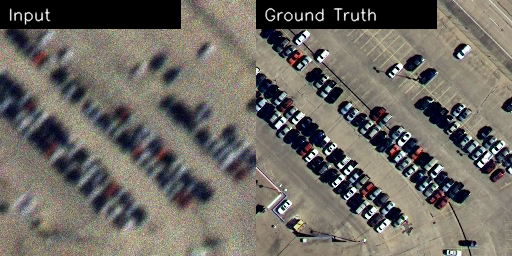
\includegraphics[width=\textwidth]{images/degradation1.png}
        \caption{Simple Parametric Degradation}
        % \caption{Typical Data Size in C}
    \end{subfigure}
    \begin{subfigure}[b]{0.45\textwidth}
        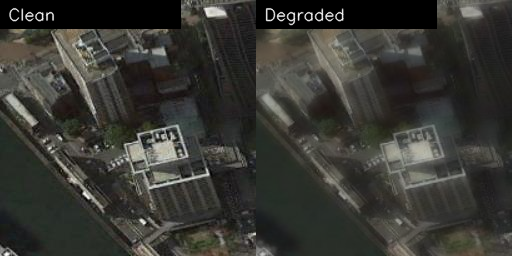
\includegraphics[width=\textwidth]{images/degradation2.png}
        \caption{Default TurbulenceSim Degradation}
        % \caption{Floating Point Representation}
    \end{subfigure}
    \caption{Comparison of two degradation pipelines.}
    \label{fig:degradation}
\end{figure} 

Among different settings of TurbulenceSim parameters (especially turbulence strength), the default configuration with strength 0.5 already produces blurring and local distortion visually similar to real atmospheric turbulence. Increasing the strength to 1.0 eventually leads to severe blur and turbulence. The visualized 7-frame images with turbulence strength ranging from 0.5 to 1.0 are shown in Figure~\ref{fig:turbulence_strength}.

\begin{figure}[htbp]
    \centering
    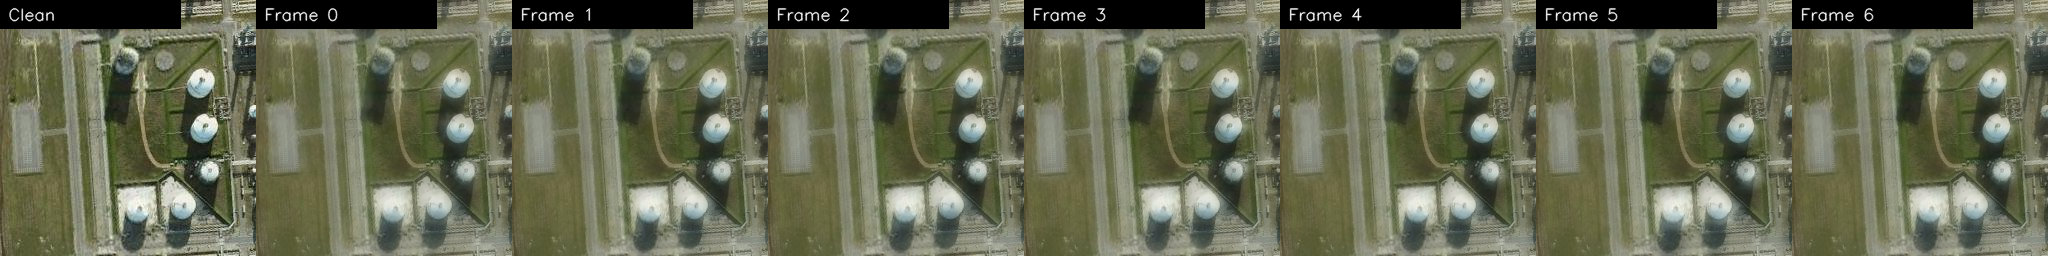
\includegraphics[width=0.9\textwidth]{images/mild50.png}
    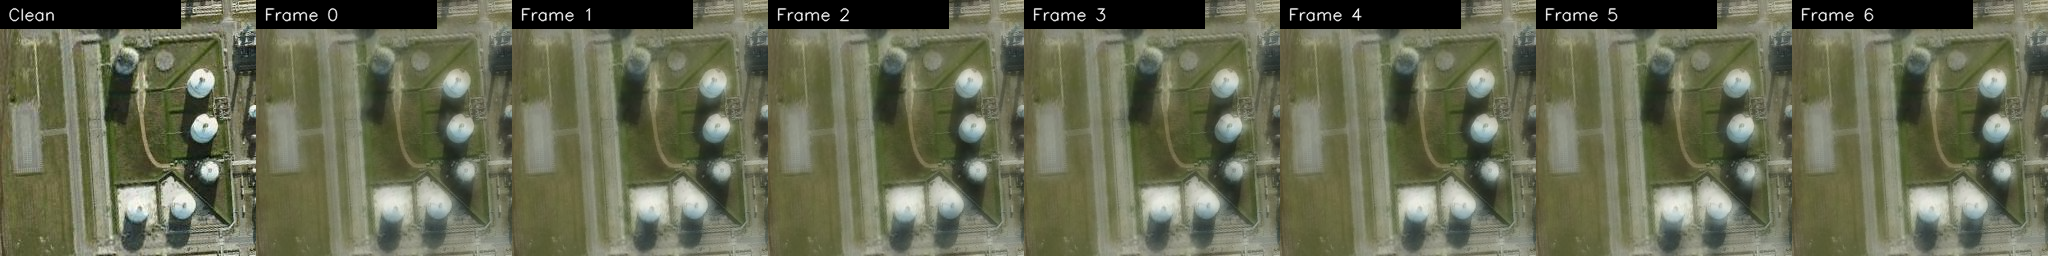
\includegraphics[width=0.9\textwidth]{images/mild60.png}
    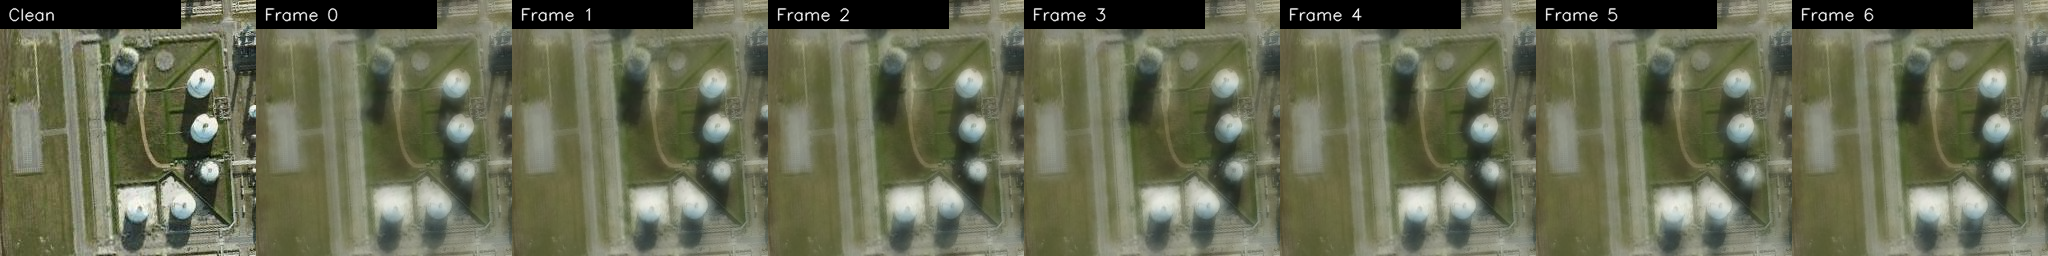
\includegraphics[width=0.9\textwidth]{images/mild70.png}
    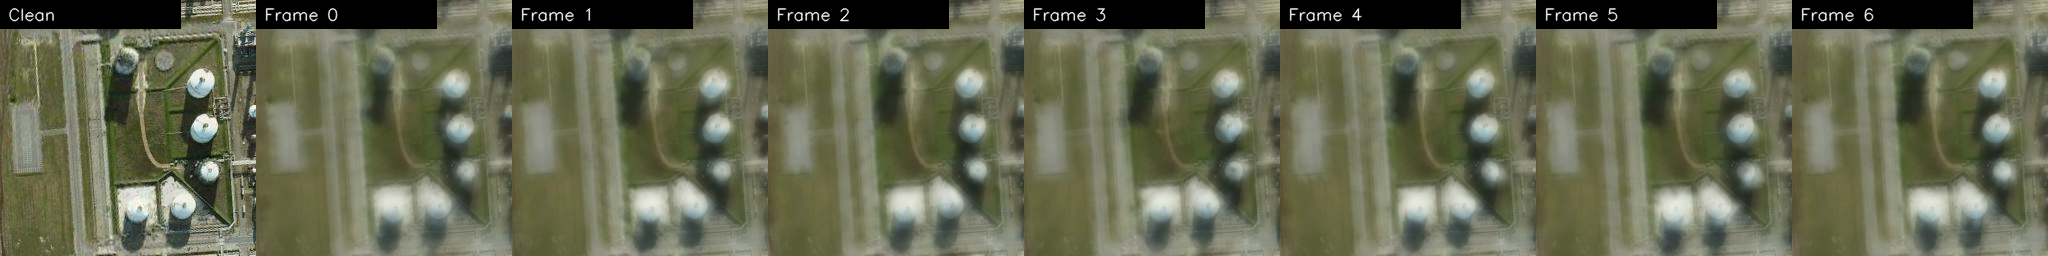
\includegraphics[width=0.9\textwidth]{images/mild80.png}
    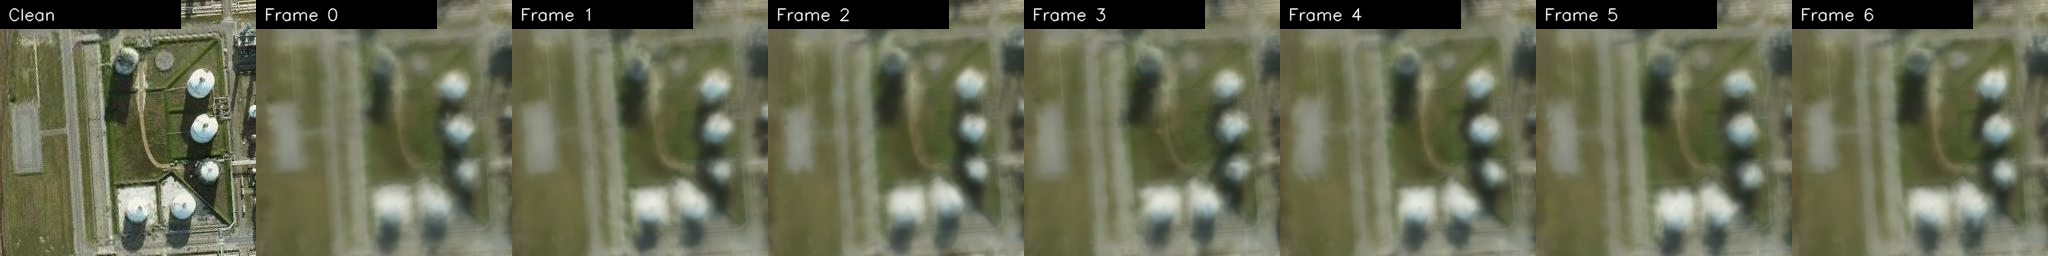
\includegraphics[width=0.9\textwidth]{images/mild90.png}
    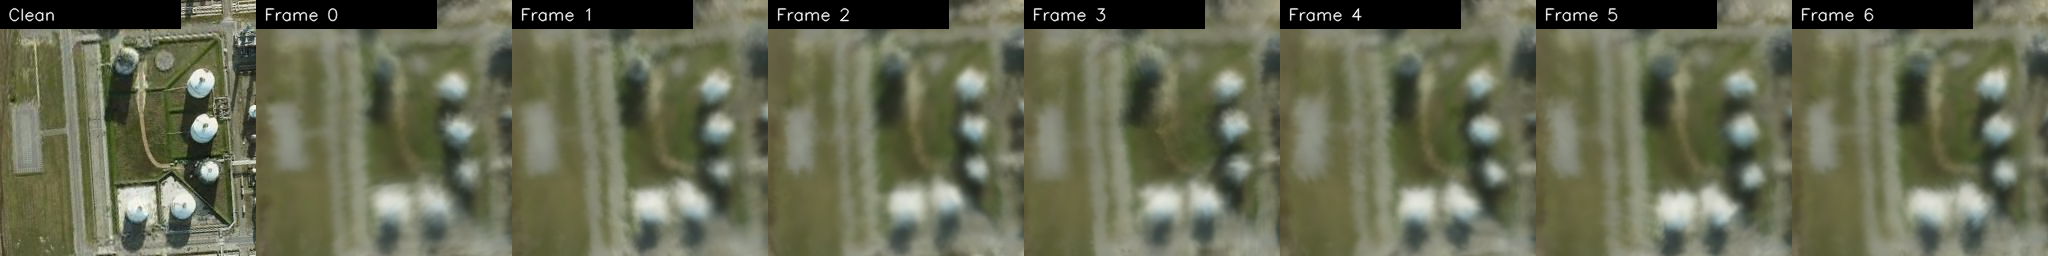
\includegraphics[width=0.9\textwidth]{images/mild100.png}
    \caption{Visualized 7-frame images with turbulence strength ranging from 0.5 to 1.0.}
    \label{fig:turbulence_strength}
\end{figure}

\subsection{Model Architecture}
\subsubsection{Multi-frame U-Net architecture baseline}
The restoration backbone is a baseline U-Net defined in the repository. It uses a standard encoder-decoder structure with four downsampling stages, four upsampling stages, skip connections, batch normalization, and ReLU activations. The base channel width is 64. Since the task is supervised image restoration, the network predicts a clean RGB image and is trained with an $L_1$ reconstruction loss.

The distinctive design choice is the input representation. Instead of restoring from a single frame, we use seven degraded frames for each sample. The training code supports several sequence-to-image adaptation strategies, and the active configuration uses channel stacking. Concretely, a sequence tensor of shape $B\times7\times3\times H\times W$ is reshaped into $B\times21\times H\times W$ before entering the network. This design is motivated by the observation that turbulence has temporal variation but also local periodicity or recurrence in distortion patterns. Multiple frames provide complementary glimpses of the clean scene: regions severely blurred in one frame may be less degraded in another. The 7-frame U-Net therefore receives a richer observation than a single-frame baseline while remaining simple enough to train stably.

With 21 input channels, 3 output channels, and base width 64, the network contains approximately 31.0 million trainable parameters. Although this is still a standard architecture rather than a specialized transformer or diffusion model, it provides a useful baseline for understanding how much performance can be extracted from physical simulation plus temporal stacking alone.

\begin{figure}[htbp]
    \centering
    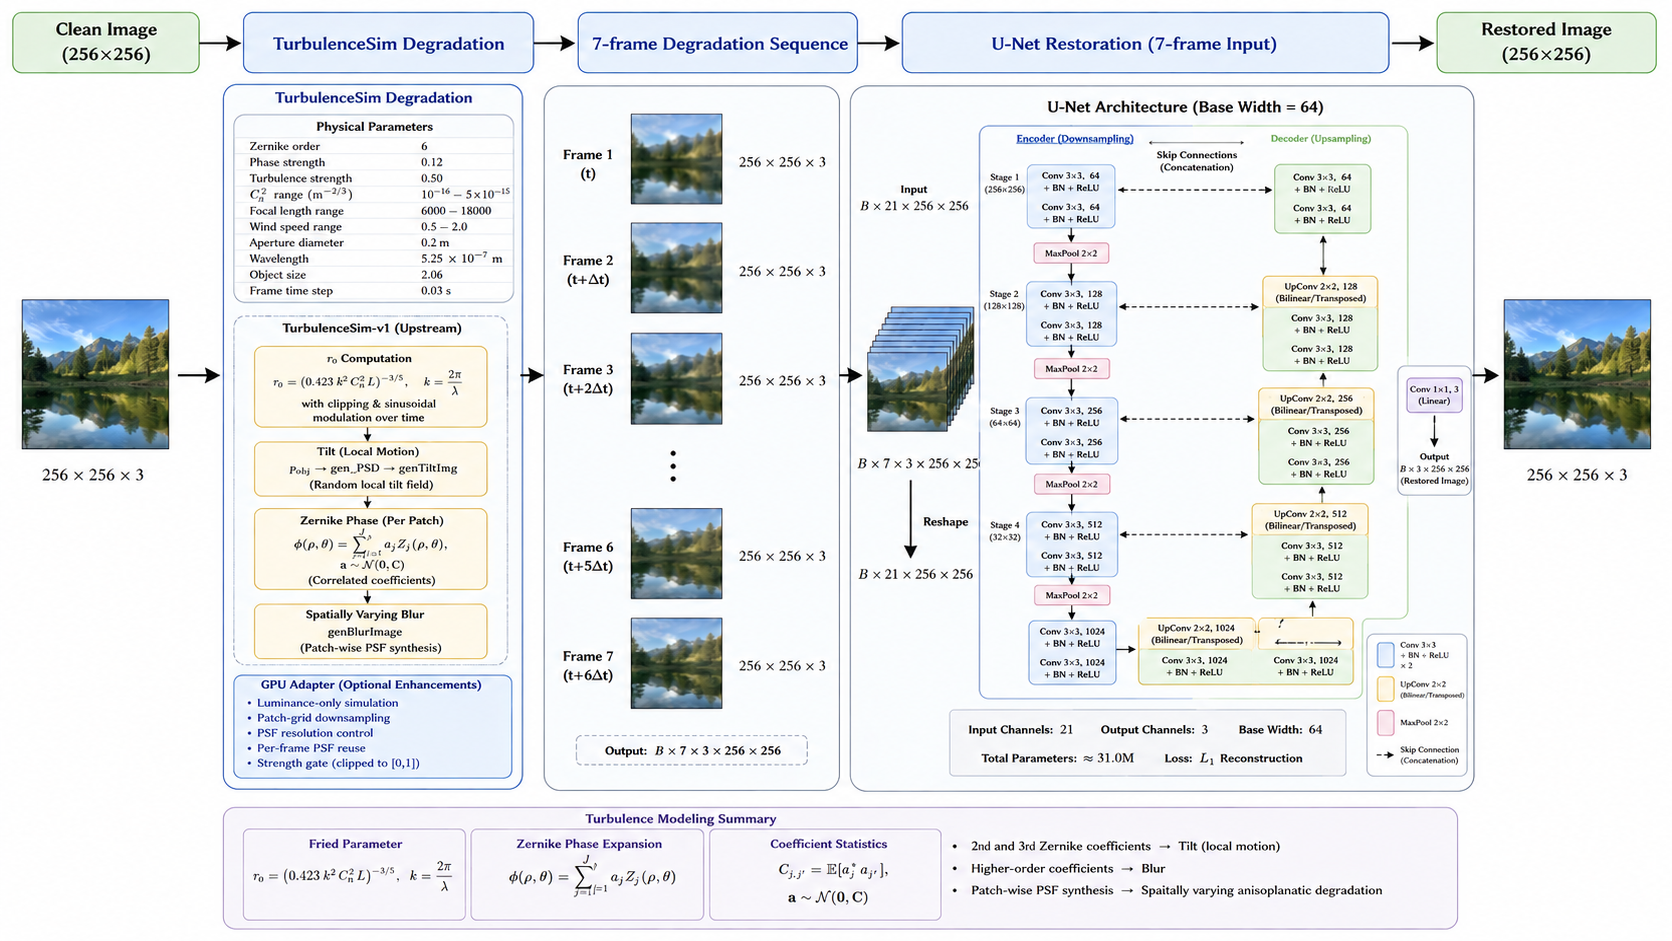
\includegraphics[width=0.9\textwidth]{images/AI-image.png}
    \caption{Schematic of the multi-frame U-Net architecture and data pipeline (GPT-image-2 generated).}
\end{figure}

\subsubsection{TSR-WGAN}
We also implement a TSR-WGAN model adapted from the turbulence sequence restoration network of Jin et al.~\citep{jin2021}. Unlike the U-Net baseline, which stacks all seven frames directly as 21 image channels, TSR-WGAN keeps the input as a sequence tensor $B\times7\times3\times H\times W$ and explicitly separates per-frame feature alignment, temporal integration, image reconstruction, and adversarial scoring. In the active configuration, the generator has approximately 46.0 million trainable parameters and the critic has approximately 1.7 million trainable parameters.

\begin{figure}[htbp]
    \centering
    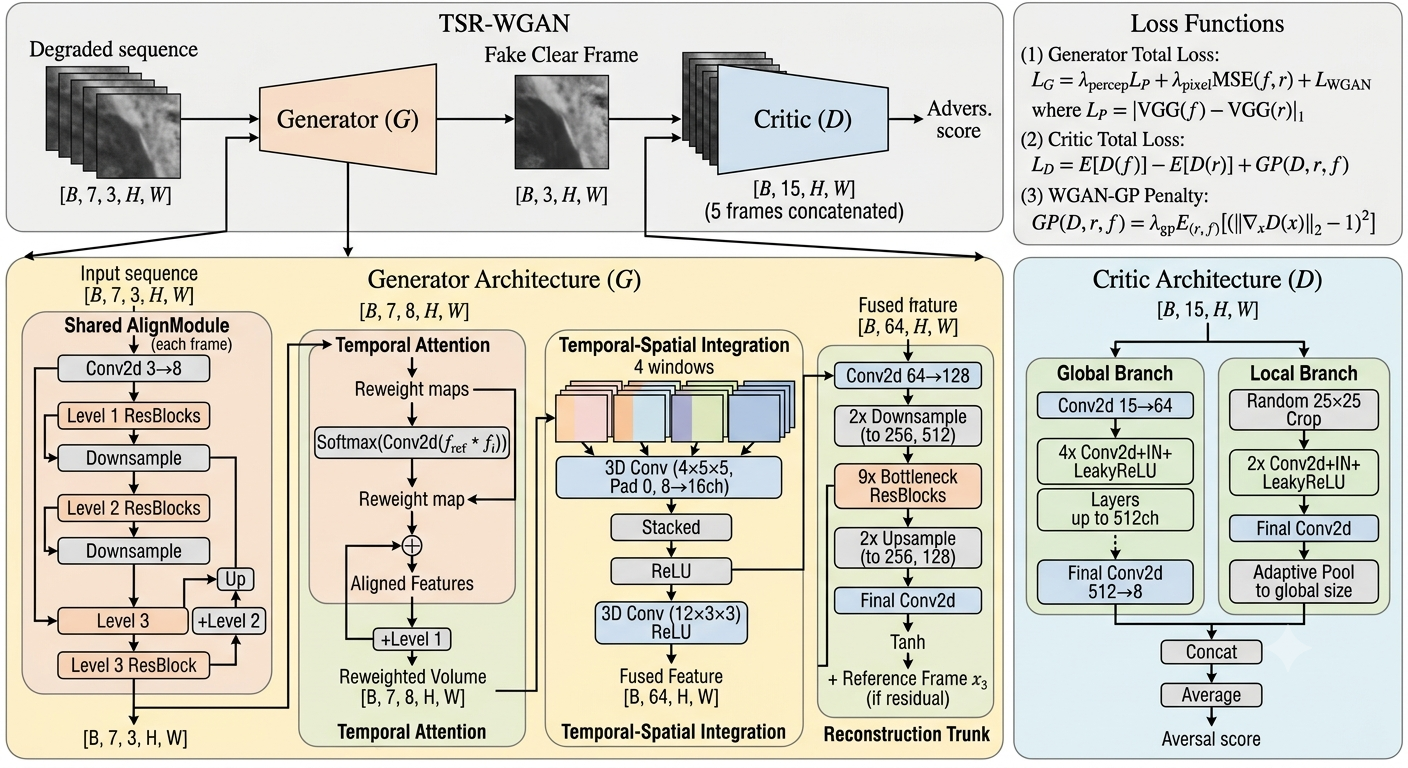
\includegraphics[width=0.9\textwidth]{images/WGAN.png}
    \caption{Schematic of the TSR-WGAN architecture and data pipeline (Nano Banana 2 generated).}
\end{figure}

The generator first applies a shared per-frame alignment module to each RGB frame. This module maps each frame from 3 channels to 8 feature channels with a $3\times3$ convolution and then builds a three-level feature pyramid. The first level operates at the original resolution, the second and third levels are produced by stride-2 $3\times3$ convolutions, and residual blocks with instance normalization refine the features at each level. Coarser features are bilinearly upsampled and added back into finer levels, so the final aligned feature for each frame remains an 8-channel full-resolution map.

After alignment, the generator uses the middle frame as the temporal reference. For every neighboring frame, the code multiplies its aligned feature with the center-frame feature, passes the product through a $7\times7$ convolution, and applies a channel-wise softmax to obtain a correlation map. The aligned feature sequence is then reweighted by these maps, which gives the generator a lightweight temporal attention mechanism before explicit 3D integration.

The temporal-spatial integration block receives the reweighted feature volume. With seven input frames, it uses four overlapping temporal windows of length four. Each window is processed by a padded $3$D convolution with kernel size $4\times5\times5$, producing 16-channel features. The four outputs are concatenated along the temporal axis and fused by another $3$D convolution whose temporal kernel spans the concatenated sequence, producing a $64\times H\times W$ representation. The reconstruction trunk then applies a $7\times7$ convolution from 64 to 128 channels, two stride-2 downsampling stages to 256 and 512 channels, nine residual blocks at the bottleneck, two transposed-convolution upsampling stages back to 128 channels, and a final $7\times7$ convolution to RGB. The model learns a residual correction: the reconstructed output is added to the center degraded frame and passed through a \texttt{tanh} activation.

The critic scores a five-frame clip centered in the seven-frame sequence. For a real clip, the center degraded frame is replaced by the clean target; for a fake clip, it is replaced by the generator output. The selected five RGB frames are flattened to 15 channels. The critic has a global branch with repeated stride-2 convolutions up to 512 channels followed by an 8-channel score map, and a local branch that crops a random $25\times25$ patch, applies two stride-2 convolutions and a final convolution to produce a local score map. The local map is adaptively pooled to the global-map size, concatenated with the global output, and averaged by the WGAN loss.



\subsection{Objectives and training details}
\subsubsection{Metrics and objective}
Training follows the implementation in \texttt{train\_unet.py}: the model predicts a restored RGB image, the prediction is clamped to $[0,1]$ before loss evaluation, and the optimization objective is the mean $L_1$ reconstruction loss against the clean target. For a minibatch of size $B$, with prediction $\hat{y}_i$ and clean target $y_i$, the loss used in training is
\begin{equation}
\mathcal{L}_{L_1}
= \frac{1}{B} \sum_{i=1}^{B} \frac{1}{CHW}
\sum_{c=1}^{C} \sum_{h=1}^{H} \sum_{w=1}^{W}
\left|\mathrm{clip}(\hat{y}_i)_{c,h,w} - y_{i,c,h,w}\right|,
\end{equation}
where $\mathrm{clip}(\cdot)$ truncates each predicted pixel to the interval $[0,1]$. During validation, the code computes batch-level PSNR and SSIM on the clamped predictions in the same $[0,1]$ range, using the full RGB image with channel-aware SSIM from \texttt{skimage}. The resulting metrics are averaged over the validation set, and checkpoint selection is based on validation PSNR. An optional LPIPS term is also implemented in the metric wrapper, but it is disabled in the default configuration.

PSNR provides a simple error-based quality score. With images normalized to $[0,1]$, it is computed from the mean squared error as
\begin{equation}
\mathrm{MSE}(y,\hat{y}) = \frac{1}{CHW}\sum_{c=1}^{C}\sum_{h=1}^{H}\sum_{w=1}^{W}(y_{c,h,w}-\hat{y}_{c,h,w})^2,
\qquad
\mathrm{PSNR}(y,\hat{y}) = 10\log_{10}\!\left(\frac{1}{\mathrm{MSE}(y,\hat{y})}\right),
\end{equation}
so higher values indicate smaller pixel-wise distortion. SSIM, following Wang et al.~\citep{wang2004ssim}, is designed to better reflect perceptual structure by comparing local luminance, contrast, and structural consistency rather than only raw error. For two local patches $x$ and $y$, the classic SSIM form is
\begin{equation}
\mathrm{SSIM}(x,y)
= \frac{(2\mu_x\mu_y + c_1)(2\sigma_{xy} + c_2)}{(\mu_x^2 + \mu_y^2 + c_1)(\sigma_x^2 + \sigma_y^2 + c_2)},
\end{equation}
where $\mu_x$ and $\mu_y$ are local means, $\sigma_x^2$ and $\sigma_y^2$ are local variances, $\sigma_{xy}$ is local covariance, and $c_1,c_2$ are stabilizing constants. In this report, PSNR is used as the primary selection metric, while SSIM is reported to summarize structural fidelity.

For TSR-WGAN, training follows the WGAN-GP formulation \citep{arjovsky2017wgan,gulrajani2017wgangp}. Let $s$ denote a seven-frame degraded sequence, $x$ the clean target, $\hat{x}=G(s)$ the generated restoration, and $\mathcal{C}(s,z)$ the five-frame critic input formed by replacing the center frame of the selected degraded clip with image $z$ and flattening the clip into 15 channels. The critic compares the real input $\mathcal{C}(s,x)$ against the fake input $\mathcal{C}(s,\hat{x})$. Its loss is
\begin{equation}
\mathcal{L}_D
= \mathbb{E}\left[D(\mathcal{C}(s,\hat{x}))\right]
- \mathbb{E}\left[D(\mathcal{C}(s,x))\right]
+ \lambda_{gp}\,\mathbb{E}_{\tilde{c}}
\left[\left(\left\|\nabla_{\tilde{c}}D(\tilde{c})\right\|_2 - 1\right)^2\right],
\end{equation}
where $\tilde{c}=\alpha\mathcal{C}(s,x)+(1-\alpha)\mathcal{C}(s,\hat{x})$ and $\alpha\sim U(0,1)$. The generator combines the adversarial term, a VGG19 perceptual loss, and a pixel MSE term:
\begin{equation}
\mathcal{L}_G
= -\mathbb{E}\left[D(\mathcal{C}(s,\hat{x}))\right]
+ \lambda_{perc}\left\|\Phi(\hat{x})-\Phi(x)\right\|_1
+ \lambda_{pix}\left\|\hat{x}-x\right\|_2^2,
\end{equation}
where $\Phi$ denotes frozen VGG19 features up to layer 14. In the active configuration, $\lambda_{gp}=10$, $\lambda_{perc}=10$, and $\lambda_{pix}=10000$. TSR-WGAN is trained and scored in the normalized $[-1,1]$ range, then converted back to $[0,1]$ for PSNR and SSIM.

\subsubsection{Training details}
Training is launched through the unified script but dispatched to model-specific entry points. For the U-Net experiments, the optimizer is Adam with learning rate 2\,$\times$\,$10^{-4}$, $\beta_1=0.5$, $\beta_2=0.999$, and zero weight decay. A StepLR scheduler halves the learning rate every 30 epochs. The U-Net models are trained for 50 epochs using automatic mixed precision when CUDA is available. The per-process training batch size is 64 and validation batch size is 8.

For TSR-WGAN, the configuration balances the mild50 and mild75 LMDB training roots and uses a sequence tensor input. The generator optimizer is Adam with learning rate 3\,$\times$\,$10^{-4}$, while the critic optimizer uses learning rate 1\,$\times$\,$10^{-5}$; both use $\beta_1=0.9$, $\beta_2=0.999$, and zero weight decay. One critic update is performed for each generator update. The model is trained for 30 epochs with batch size 12 and validation batch size 12. Mixed precision is disabled in this path because WGAN-GP gradient penalty training is unstable under automatic mixed precision. A ReduceLROnPlateau scheduler is enabled for both optimizers with factor 0.5 and patience 5.

The code also supports distributed data parallel training through torchrun. When launched with multiple GPUs, the project initializes an NCCL process group, assigns one GPU per process, uses distributed samplers, and aggregates metrics across ranks. This is especially relevant for the current setting because sequence inputs increase memory pressure compared with single-frame restoration. For all reported checkpoints, model selection is based on validation PSNR.

\section{Results and Analysis}
\subsection{Quantitative results}
\subsubsection{Validation performance}
The best U-Net and TSR-WGAN checkpoints evaluated on the validation split reach the metrics shown in Table~\ref{tab:quantitative}. The reported values come from the repository output generated by the evaluation pipeline.

\begin{table}[H]
    \centering
    \caption{Validation performance of the U-Net and TSR-WGAN restoration models.}
    \label{tab:quantitative}
    \begin{tabular}{lcccc}
        \toprule
        Model & Input setting & Data turbulence strength & PSNR $\uparrow$ & SSIM $\uparrow$ \\
        \midrule
        U-Net baseline & 7 frames stacked & 0.5 & 35.341 & 0.9804 \\
        U-Net baseline & 1 frame & 0.5 & 31.483 & 0.9581 \\
        U-Net baseline & 7 frames stacked & 0.75 & 31.783 & 0.9557 \\
        U-Net baseline & 1 frame & 0.75 & 29.463 & 0.9256 \\
        TSR-WGAN & 7 frames sequence & mixed 0.5/0.75 & 34.144 & 0.9712 \\
        \bottomrule
    \end{tabular}
\end{table}

The absolute values indicate that both model families recover a large portion of the structural signal from the simulated degradation. A PSNR above 35 dB for the best U-Net on 256\,$\times$\,256 remote sensing patches suggests that the network is not merely smoothing the image, but is reconstructing scene content in a way that remains close to the clean target. TSR-WGAN reaches a slightly lower but still strong validation score of 34.144 dB PSNR and 0.9712 SSIM, which is notable because it is trained on a mixed 0.50/0.75 turbulence distribution rather than a single mild setting.

At the same time, these numbers should be interpreted carefully. The evaluation uses synthetic degradations drawn from the same simulator family as training, so the results primarily measure how well the network learns to invert the chosen physical data model. They do not yet guarantee the same level of performance on real atmospheric turbulence data. This gap between simulated and real degradation remains one of the key limitations of turbulence restoration research. We will dive deeper into this issue in the following parts.

\subsubsection{Generalization across input settings and turbulence strengths}
We also studied the generalization ability of the baseline U-Net model trained on 7-frame input of 0.5 turbulence strength by testing it on both single-frame and seven-frame inputs with different turbulence strength ranging from 0.5 to 1.0. The metrics are shown in Table~\ref{tab:generalization} and Figure~\ref{fig:generalization}. 

% strength_percent,turbulence_strength,psnr_single,ssim_single,psnr_seven,ssim_seven
% 50,0.5,30.205673,0.962571,33.097409,0.979393
% 55,0.55,29.118204,0.95247,31.918176,0.973277
% 60,0.6,27.762056,0.934387,30.18827,0.959298
% 65,0.65,26.37806,0.907054,28.435685,0.936001
% 70,0.7,25.070179,0.869362,26.83019,0.902037
% 75,0.75,23.869369,0.820553,25.398539,0.85637
% 80,0.8,22.779796,0.760534,24.129658,0.798524
% 85,0.85,21.791512,0.689837,23.000419,0.728735
% 90,0.9,20.894364,0.61009,21.989839,0.648349
% 95,0.95,20.076583,0.523661,21.078343,0.559506
% 100,1.0,19.324775,0.433028,20.249447,0.465067

The results show that the 7-frame U-Net model trained on 7-frame input can generalize to single-frame input only with a performance drop of approximately 2 dB in PSNR and 0.02 in SSIM across different turbulence strengths. This suggests that the model has learned some robust features that are not entirely dependent on the multi-frame input, but the performance gap also indicates that the temporal information from multiple frames is valuable for achieving higher restoration quality.

However, the performance drops significantly as turbulence strength increases both for single-frame and multi-frame inputs, which is expected since stronger turbulence degradation leaves less information available and is more challenging to restore.

\begin{table}[H]
    \centering
    \caption{Generalization performance of the 7-frame U-Net model trained on 0.50 turbulence strength across different turbulence strengths and input settings.}
    \label{tab:generalization}
    \begin{tabular}{lcccc}
        \toprule
        Turbu-strength & PSNR (1 frame) $\uparrow$ & SSIM (1 frame) $\uparrow$ & PSNR (7 frames) $\uparrow$ & SSIM (7 frames) $\uparrow$ \\
        \midrule
        0.5 & \textbf{30.21} & \textbf{0.9626} & \textbf{33.10} & \textbf{0.9794} \\
        0.55 & 29.12 & 0.9525 & 31.92 & 0.9733 \\
        0.6 & 27.76 & 0.9344 & 30.19 & 0.9593 \\
        0.65 & 26.38 & 0.9071 & 28.44 & 0.9360 \\
        0.7 & 25.07 & 0.8694 & 26.83 & 0.9020 \\
        0.75 & 23.87 & 0.8206 & 25.40 & 0.8564 \\
        0.8 & 22.78 & 0.7605 & 24.13 & 0.7985 \\
        0.85 & 21.79 & 0.6898 & 23.00 & 0.7287 \\
        0.9 & 20.89 & 0.6101 & 21.99 & 0.6483 \\
        0.95 & 20.08 & 0.5237 & 21.08 & 0.5595 \\
        1.0 & 19.32 & 0.4330 & 20.25 & 0.4651 \\
        \bottomrule
    \end{tabular}
\end{table}

\begin{figure}[H]
    \centering
    \begin{subfigure}[b]{0.49\textwidth}
        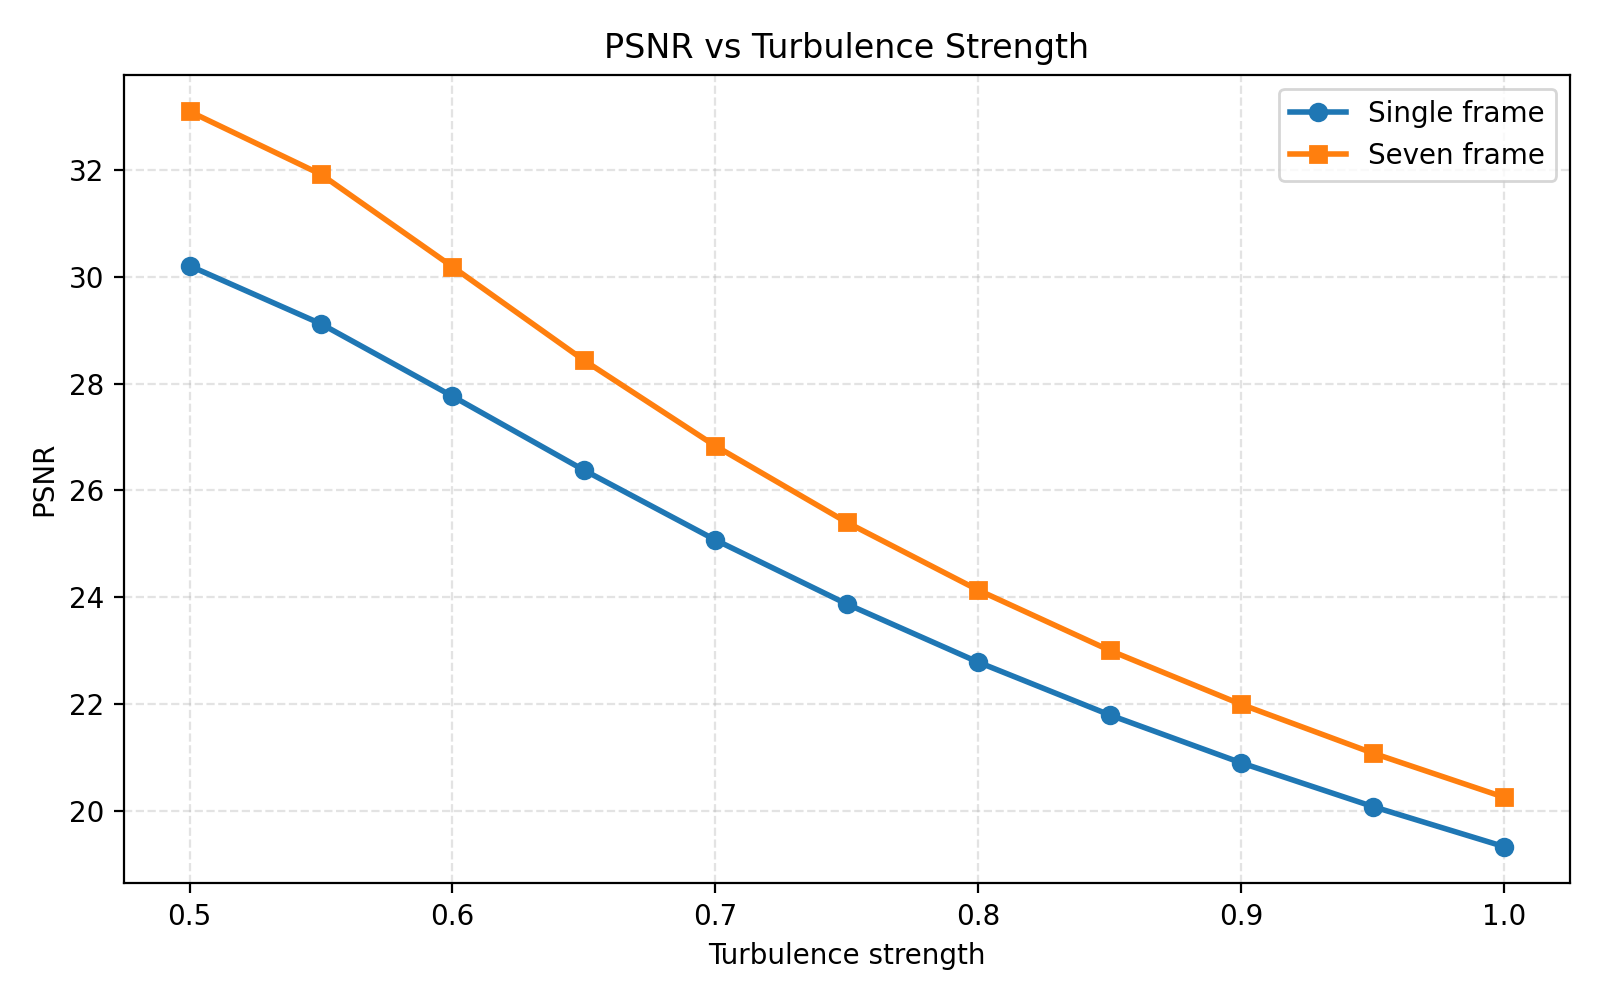
\includegraphics[width=\textwidth]{images/psnr_vs_turbulence_strength.png}
        \caption{PSNR across turbulence strengths.}
    \end{subfigure}
    \begin{subfigure}[b]{0.49\textwidth}
        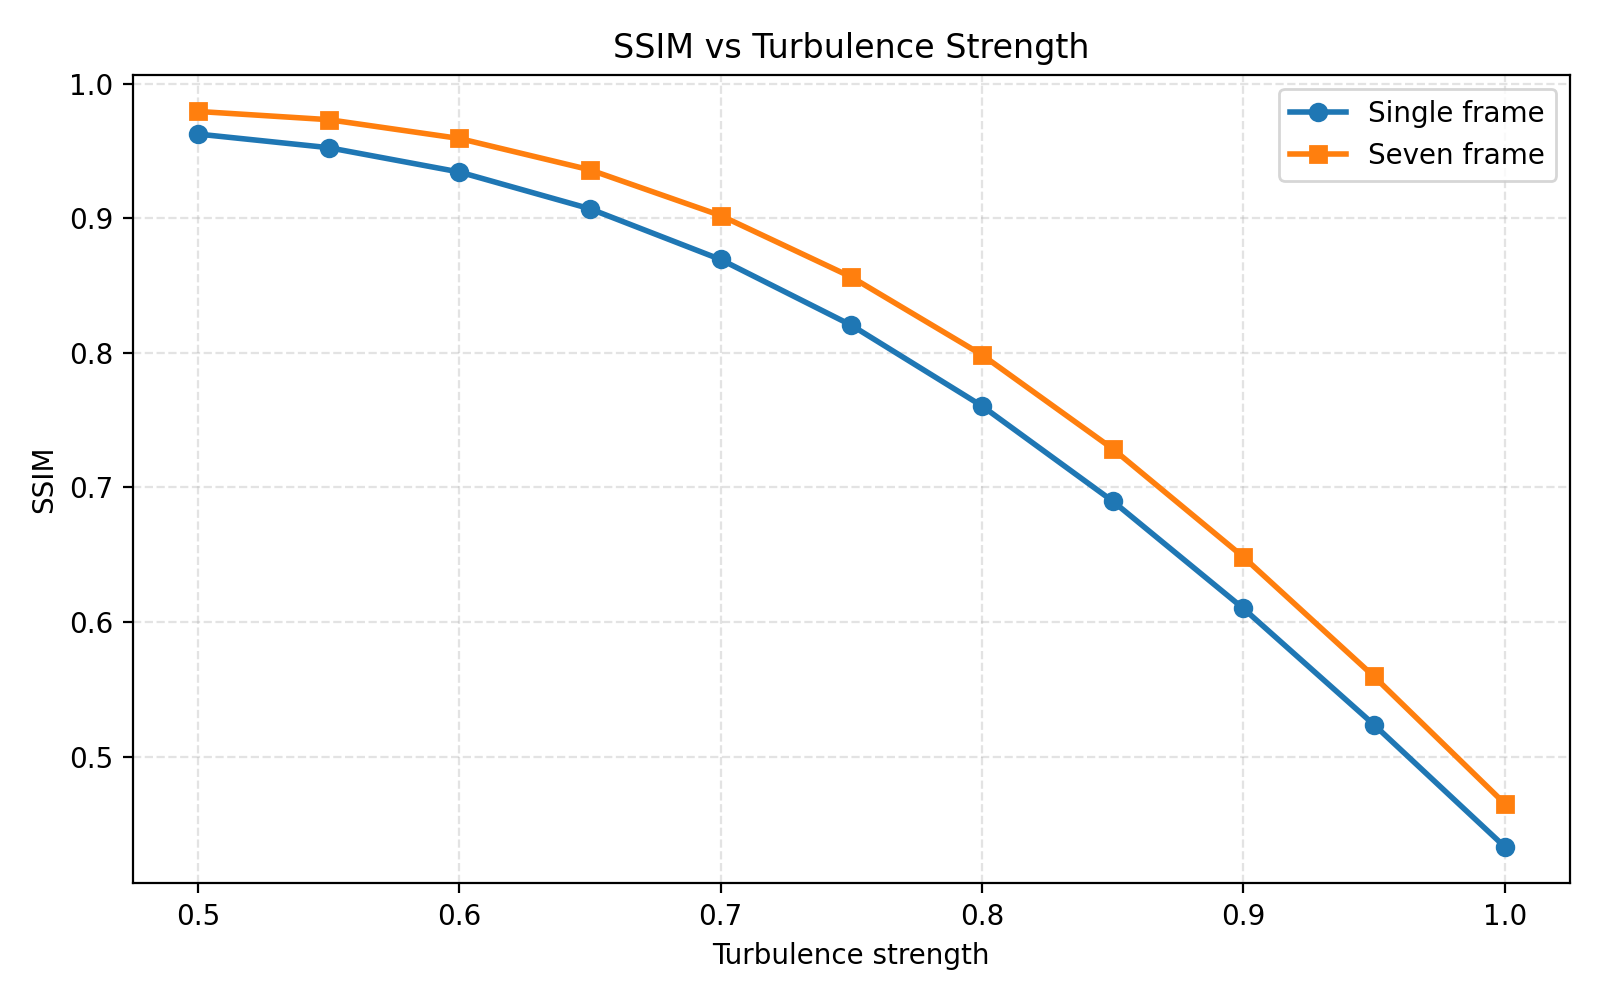
\includegraphics[width=\textwidth]{images/ssim_vs_turbulence_strength.png}
        \caption{SSIM across turbulence strengths.}
    \end{subfigure}
    \caption{Generalization performance of the 7-frame U-Net model trained on 0.50 turbulence strength across different turbulence strengths and input settings.}
    \label{fig:generalization}
\end{figure}

However, when we studied the generalization performance of the 7-frame U-Net model trained on 0.75 turbulence strength, the metrics are not monotonically decreasing as turbulence strength increases. The metrics are shown in Table~\ref{tab:generalization75} and Figure~\ref{fig:generalization75}. 

% strength_percent,turbulence_strength,psnr_single,ssim_single,psnr_seven,ssim_seven
% 50,0.5,23.299064,0.848514,23.831587,0.863411
% 55,0.55,24.229634,0.869547,25.119061,0.889906
% 60,0.6,25.116325,0.887178,26.604572,0.914462
% 65,0.65,25.762615,0.898752,28.150096,0.934519
% 70,0.7,25.869441,0.900297,29.237498,0.945979
% 75,0.75,25.268695,0.886362,28.990389,0.942874
% 80,0.8,24.128527,0.850463,27.399049,0.917162
% 85,0.85,22.759442,0.78587,25.395812,0.860031
% 90,0.9,21.383356,0.688954,23.496644,0.764942
% 95,0.95,20.102179,0.562549,21.821909,0.632463
% 100,1.0,18.941284,0.417077,20.368315,0.473462

\begin{table}[H]
    \centering
    \caption{Generalization performance of the 7-frame U-Net model trained on 0.75 turbulence strength across different turbulence strengths and input settings.}
    \label{tab:generalization75}
    \begin{tabular}{lcccc}
        \toprule
        Turbu-strength & PSNR (1 frame) $\uparrow$ & SSIM (1 frame) $\uparrow$ & PSNR (7 frames) $\uparrow$ & SSIM (7 frames) $\uparrow$ \\
        \midrule
        0.5 & 23.30 & 0.8485 & 23.83 & 0.8634 \\
        0.55 & 24.23 & 0.8695 & 25.12 & 0.8899 \\
        0.6 & 25.12 & 0.8872 & 26.60 & 0.9145 \\
        0.65 & 25.76 & 0.8988 & 28.15 & 0.9345 \\
        0.7 & \textbf{25.87} & \textbf{0.9003} & \textbf{29.24} & \textbf{0.9460} \\
        0.75 & 25.27 & 0.8864 & 28.99 & 0.9429 \\
        0.8 & 24.13 & 0.8505 & 27.40 & 0.9172 \\
        0.85 & 22.76 & 0.7859 & 25.40 & 0.8600 \\
        0.9 & 21.38 & 0.6890 & 23.50 & 0.7649 \\
        0.95 & 20.10 & 0.5625 & 21.82 & 0.6325 \\
        1.0 & 18.94 & 0.4171 & 20.37 & 0.4735 \\
        \bottomrule
    \end{tabular}
\end{table}

\begin{figure}[H]
    \centering
    \begin{subfigure}[b]{0.45\textwidth}
        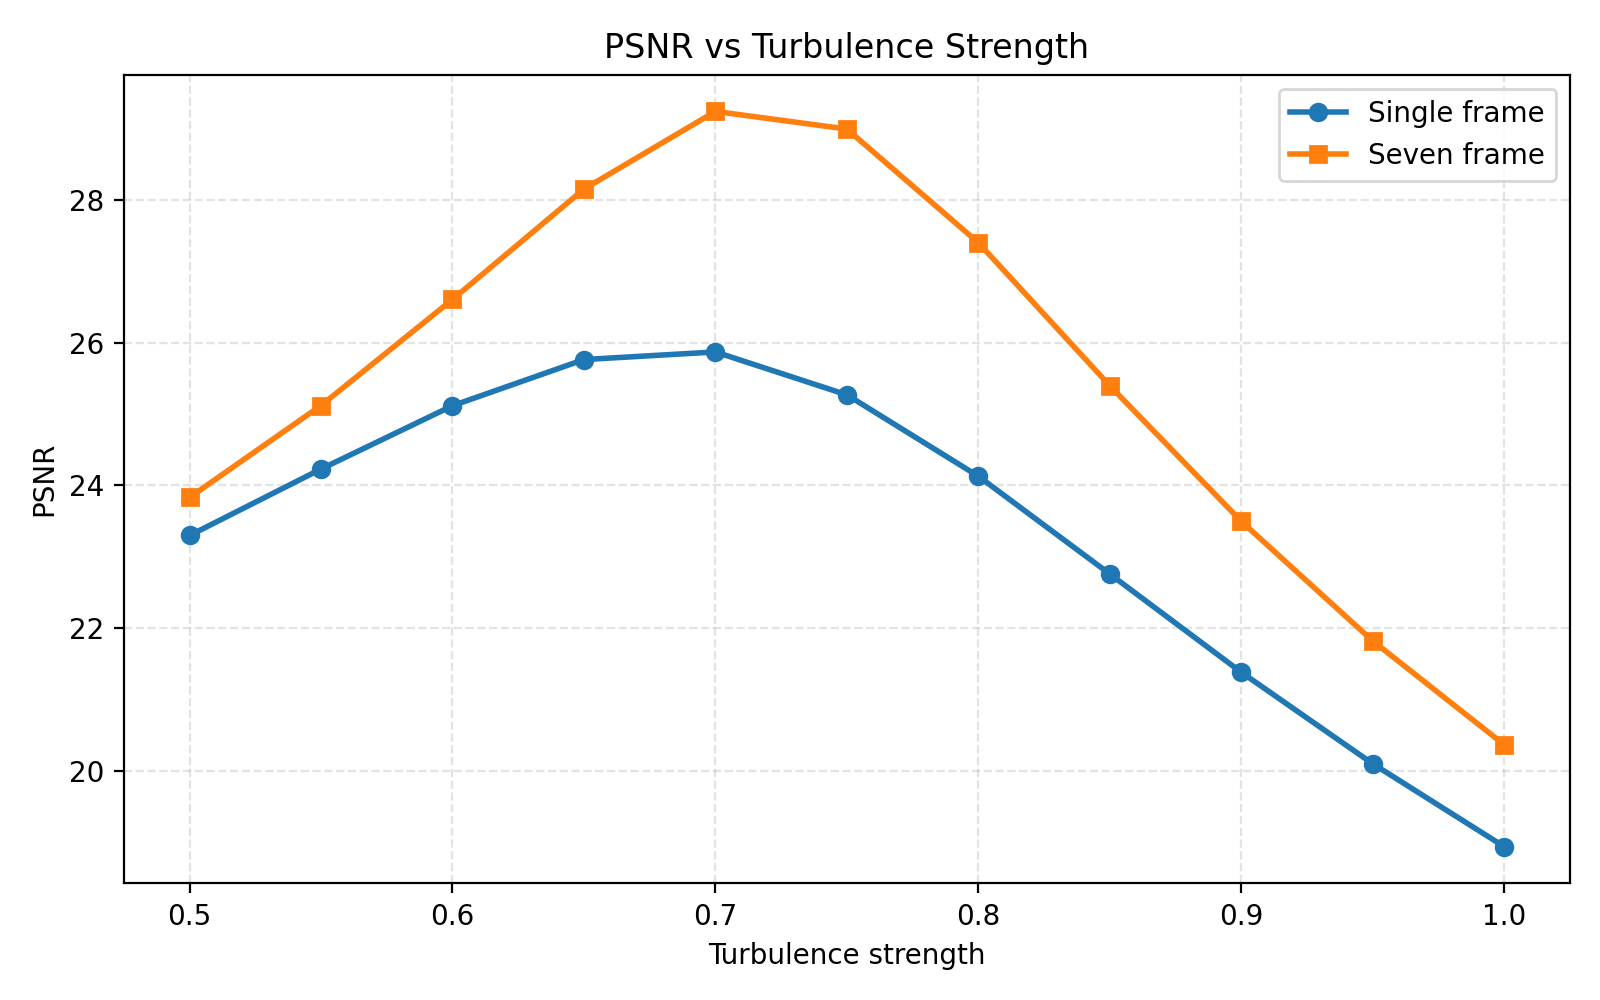
\includegraphics[width=\textwidth]{images/psnr_vs_turbulence_strength_75.png}
        \caption{PSNR across turbulence strengths.}
    \end{subfigure}
    \begin{subfigure}[b]{0.45\textwidth}
        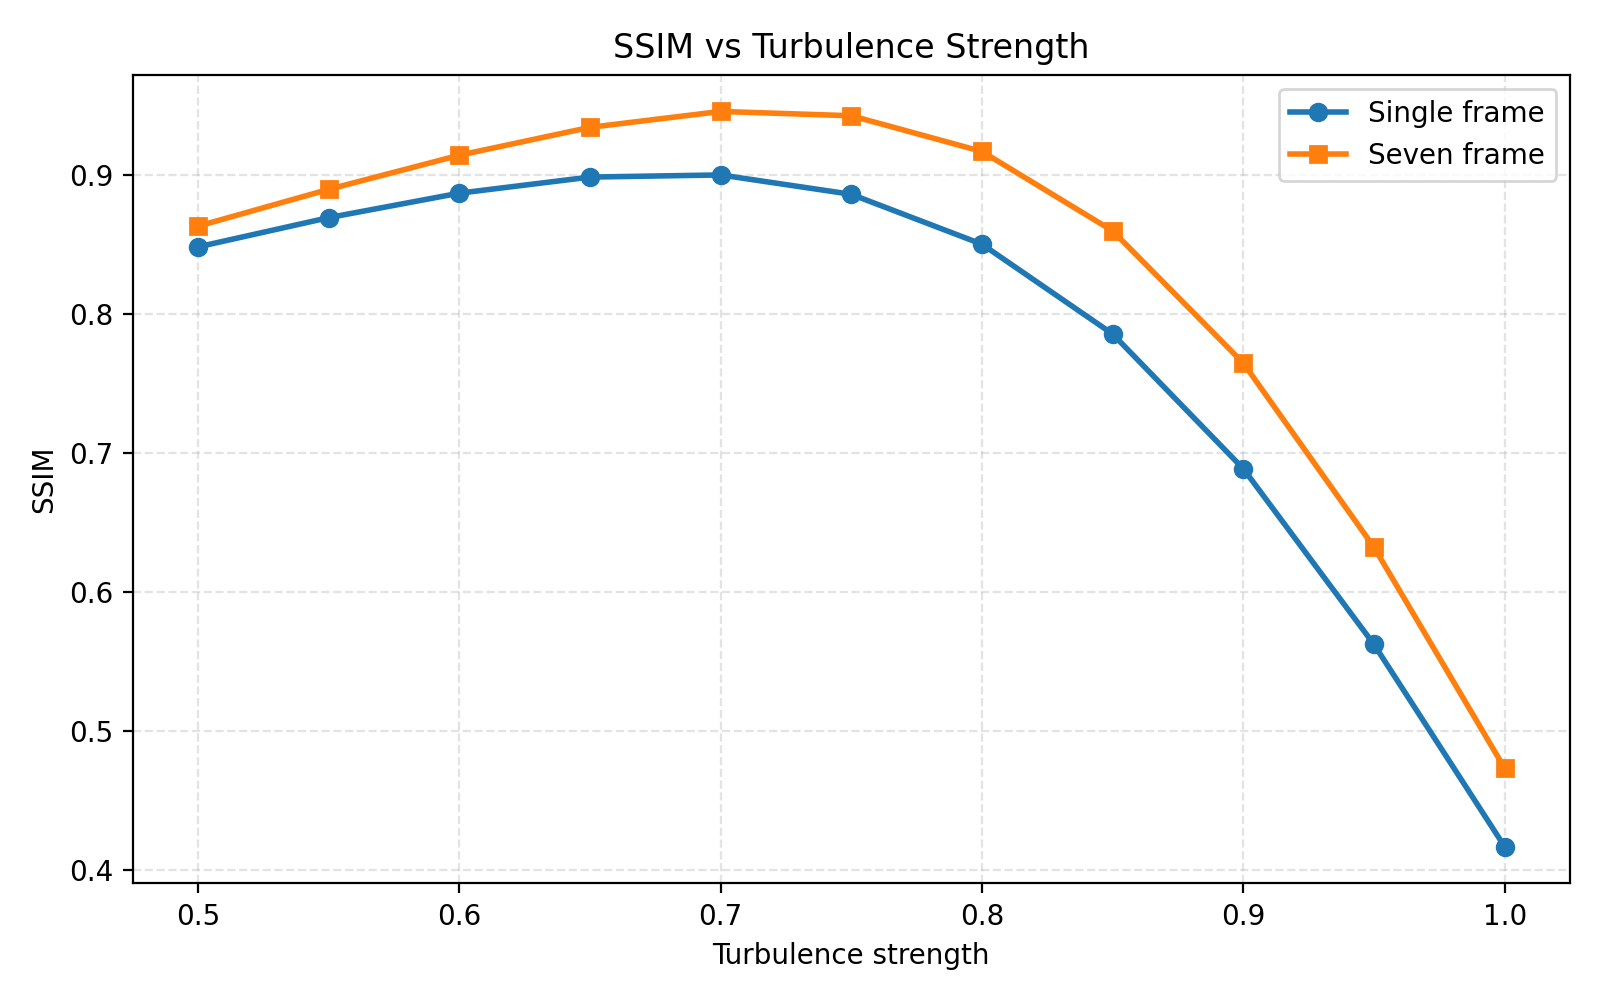
\includegraphics[width=\textwidth]{images/ssim_vs_turbulence_strength_75.png}
        \caption{SSIM across turbulence strengths.}
    \end{subfigure}
    \caption{Generalization performance of the 7-frame U-Net model trained on 0.75 turbulence strength across different turbulence strengths and input settings.}
    \label{fig:generalization75}
\end{figure}

The peak performance at 0.70 test-time turbulence strength is unexpected, showing an equilibrium between remembering the degradation distribution and easiness of restoration. For lower turbulence strength, the model may be overfitting to the stronger degradation seen in training, while for higher turbulence strength the restoration task becomes more difficult and the model's learned features may not be sufficient to recover the clean image. This non-monotonic behavior suggests that the model's generalization is influenced by a complex interplay between the training degradation distribution and the test-time degradation, which could be an interesting direction for further investigation.

Finally, we evaluate the TSR-WGAN model trained on the mixed 0.50 and 0.75 turbulence-strength datasets. The results are shown in Table~\ref{tab:generalization_tsr_wgan} and Figure~\ref{fig:generalization_tsr_wgan}. In contrast to the 0.75-trained U-Net, TSR-WGAN shows an almost monotonic decrease as test turbulence strength increases. The seven-frame input remains consistently better than the single-frame setting, and the gap becomes very large in the moderate and strong turbulence ranges: at 0.75 strength, TSR-WGAN obtains 29.69 dB with seven frames compared with 23.60 dB with a single frame. This indicates that the temporal-spatial generator and clip-based critic use sequence information more aggressively than the channel-stacked U-Net baseline.

\begin{table}[H]
    \centering
    \caption{Generalization performance of TSR-WGAN trained on mixed 0.50 and 0.75 turbulence strengths across different turbulence strengths and input settings.}
    \label{tab:generalization_tsr_wgan}
    \begin{tabular}{lcccc}
        \toprule
        Turbu-strength & PSNR (1 frame) $\uparrow$ & SSIM (1 frame) $\uparrow$ & PSNR (7 frames) $\uparrow$ & SSIM (7 frames) $\uparrow$ \\
        \midrule
        0.5 & \textbf{28.70} & \textbf{0.9421} & \textbf{32.35} & \textbf{0.9714} \\
        0.55 & 27.61 & 0.9254 & 31.86 & 0.9677 \\
        0.6 & 26.55 & 0.9041 & 31.36 & 0.9636 \\
        0.65 & 25.53 & 0.8773 & 30.84 & 0.9588 \\
        0.7 & 24.55 & 0.8439 & 30.30 & 0.9530 \\
        0.75 & 23.60 & 0.8023 & 29.69 & 0.9451 \\
        0.8 & 22.69 & 0.7510 & 28.89 & 0.9326 \\
        0.85 & 21.80 & 0.6879 & 27.71 & 0.9092 \\
        0.9 & 20.94 & 0.6118 & 25.89 & 0.8593 \\
        0.95 & 20.11 & 0.5229 & 23.21 & 0.7376 \\
        1.0 & 19.33 & 0.4257 & 20.23 & 0.4800 \\
        \bottomrule
    \end{tabular}
\end{table}

\begin{figure}[H]
    \centering
    \begin{subfigure}[b]{0.45\textwidth}
        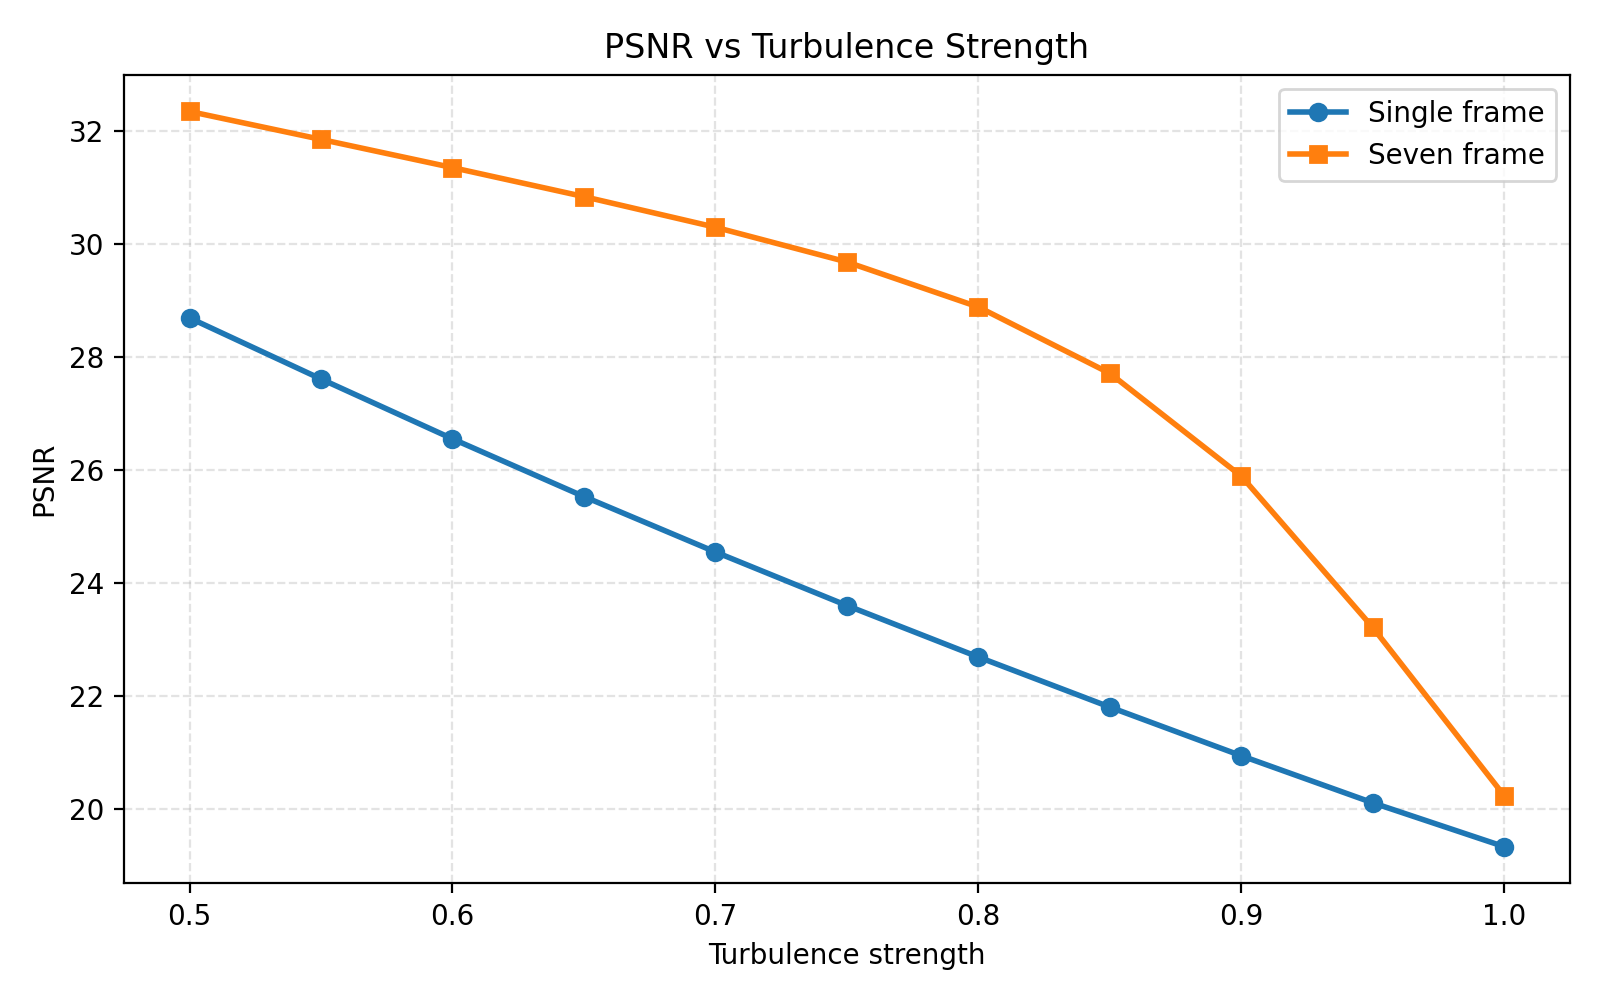
\includegraphics[width=\textwidth]{images/tsr_wgan_psnr_vs_turbulence_strength.png}
        \caption{PSNR across turbulence strengths.}
    \end{subfigure}
    \begin{subfigure}[b]{0.45\textwidth}
        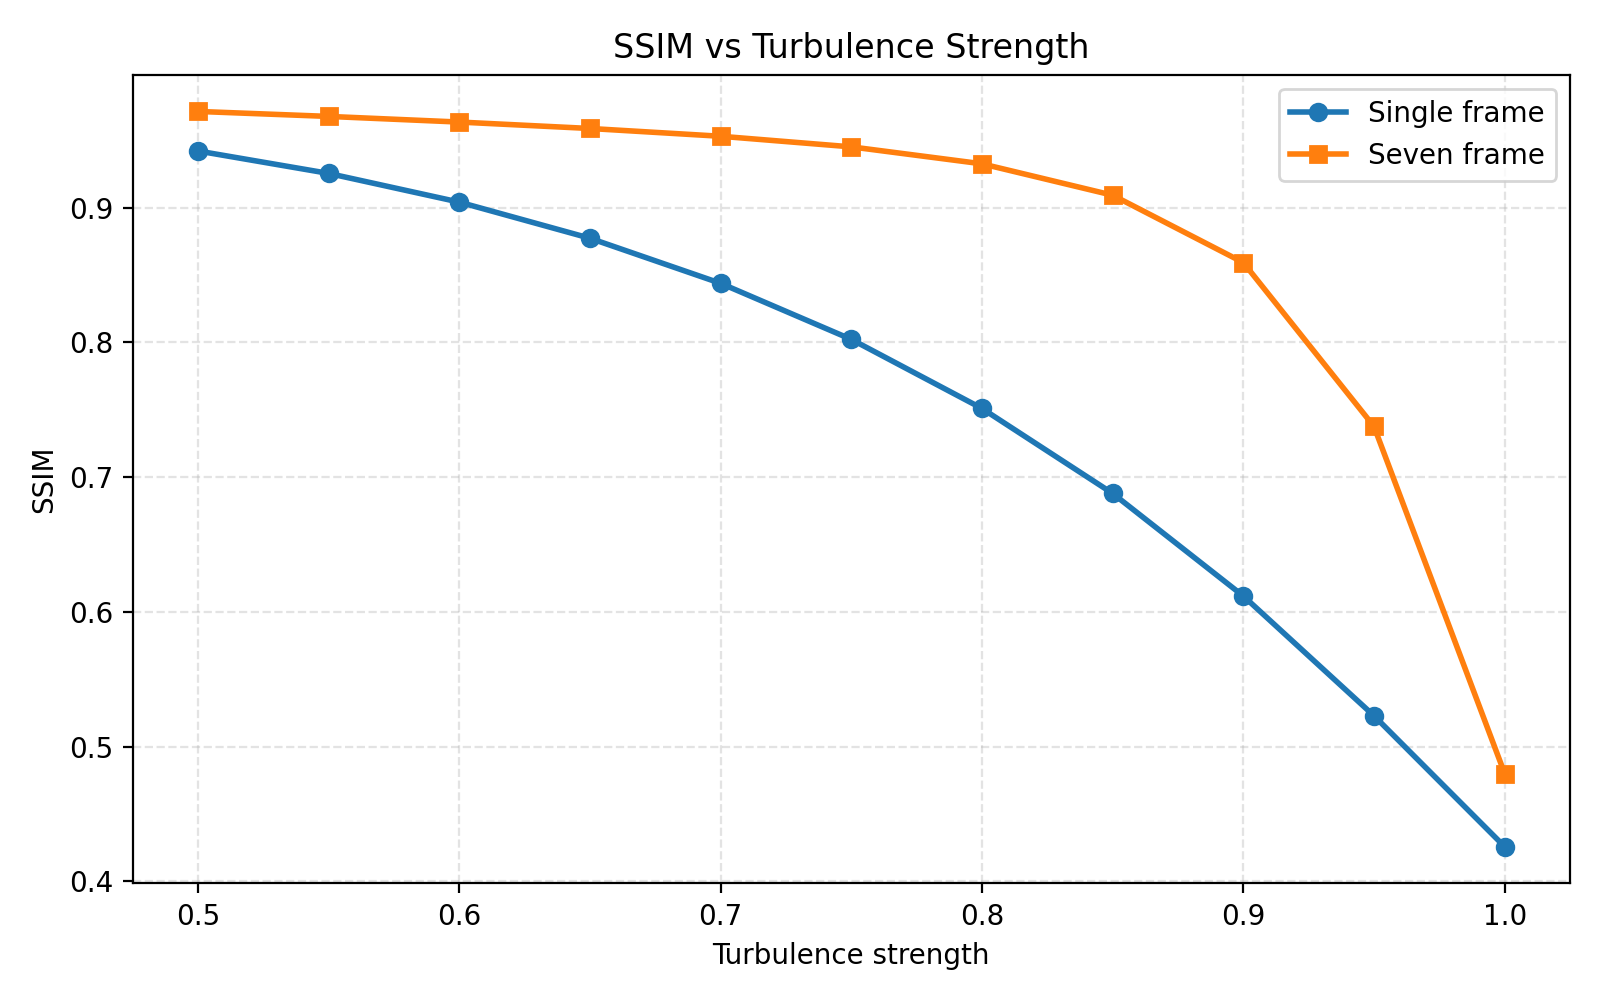
\includegraphics[width=\textwidth]{images/tsr_wgan_ssim_vs_turbulence_strength.png}
        \caption{SSIM across turbulence strengths.}
    \end{subfigure}
    \caption{Generalization performance of TSR-WGAN trained on mixed 0.50 and 0.75 turbulence strengths across different turbulence strengths and input settings.}
    \label{fig:generalization_tsr_wgan}
\end{figure}

\subsection{Qualitative results}

\begin{figure}[htbp]
    \centering
    % 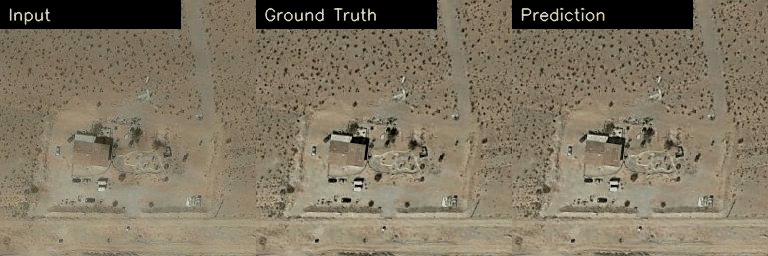
\includegraphics[width=0.88\linewidth]{images/gif00000_4.png}
    % \vspace{0.5em}
    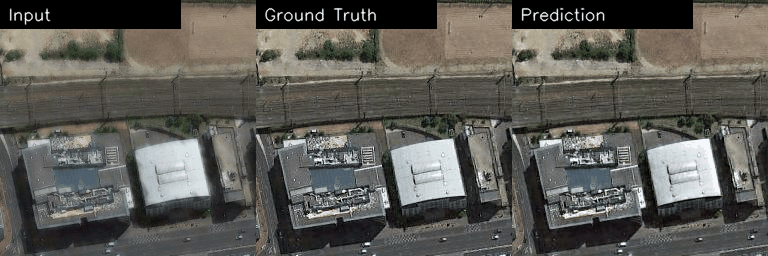
\includegraphics[width=0.8\linewidth]{images/gif00024_1.png}
    \caption{Representative restoration examples from the validation set (0.50 training time turbulence strength). From left to right in each row: degraded input, clean target, and U-Net prediction.}
    \label{fig:qualitative}
\end{figure}

Figure~\ref{fig:qualitative} shows representative restoration examples from the validation set. Each row corresponds to one sample, with the degraded input on the left, the clean target in the middle, and the U-Net prediction on the right. The visualized examples are selected to cover a range of scene types (e.g., roads, buildings, parking areas, wild areas) and to highlight typical restoration improvements. The restoration performance of default 0.50 turbulence strength is nearly perfect.

Figure~\ref{fig:qualitative75} shows representative restoration examples from the validation set with 0.75 training time turbulence strength. Compared to the generalization results in Figure~\ref{fig:generalization}, the restoration resolution is relatively high for 0.75 turbulence strength. One difference seen by naked eye is that the color saturation of the restored images are slightly lower than those of the ground truth.

\begin{figure}[htbp]
    \centering
    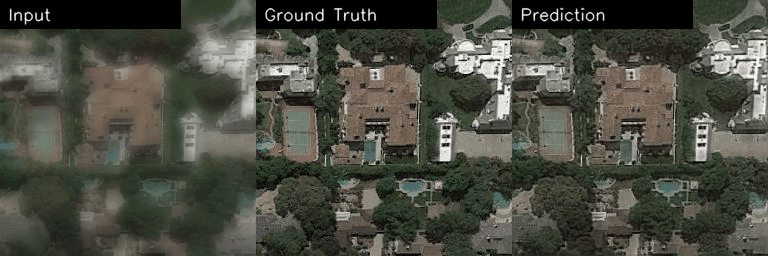
\includegraphics[width=0.8\linewidth]{images/mild75-val1.png}
    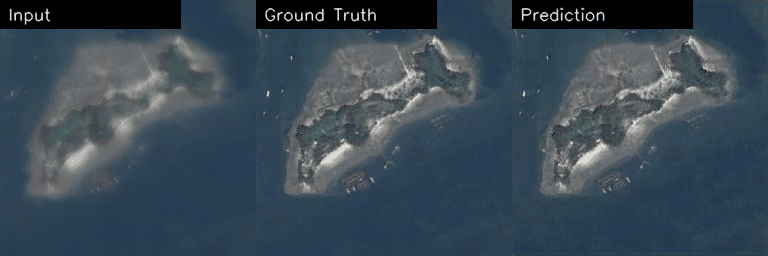
\includegraphics[width=0.8\linewidth]{images/mild75-val2.png}
    \caption{Representative restoration examples from the validation set with 0.75 training time turbulence strength. From left to right in each row: degraded input, clean target, and U-Net prediction.}
    \label{fig:qualitative75}
\end{figure}

Figure~\ref{fig:tsr_wgan_qualitative} shows a representative TSR-WGAN validation result. The prediction preserves the dominant landform boundaries and large texture regions, but the output is slightly darker and smoother than the clean target. This behavior is consistent with the quantitative result: TSR-WGAN is competitive, but its perceptual and adversarial terms do not automatically guarantee higher PSNR than the direct U-Net reconstruction objective on this simulator-domain validation split.

\begin{figure}[htbp]
    \centering
    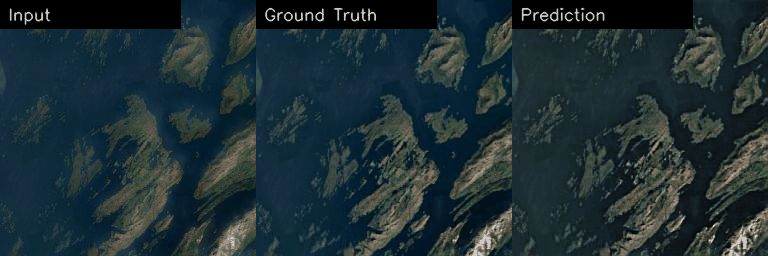
\includegraphics[width=0.8\linewidth]{images/tsr_wgan_val_00006.png}
    \caption{Representative TSR-WGAN restoration example from the validation set. From left to right: degraded input, clean target, and TSR-WGAN prediction.}
    \label{fig:tsr_wgan_qualitative}
\end{figure}

\begin{figure}[htbp]
    \centering
    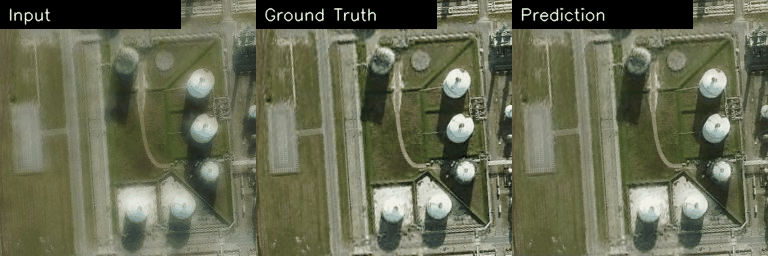
\includegraphics[width=0.8\linewidth]{images/seven6.png}
    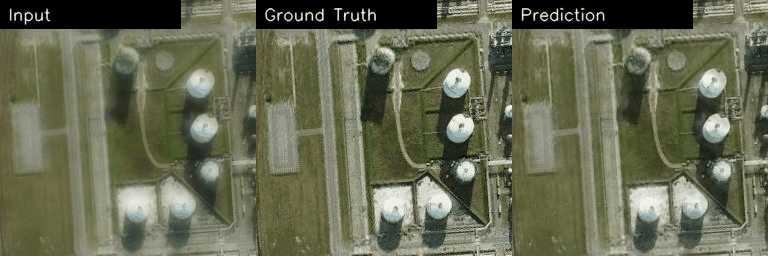
\includegraphics[width=0.8\linewidth]{images/single6.png}
    \caption{Comparison between U-Net models trained on 7-frame input (top) and 1-frame input (down) with 0.50 training time and 0.60 test time turbulence strength. }
    \label{fig:compare60}
\end{figure}
Figure~\ref{fig:compare60} shows the restoration results of the 7-frame U-Net model when test-time input is one-frame and seven-frame with turbulence strength 0.60. The results demonstrate some slight differences, e.g. the white building roof is more clearly restored in the seven-frame input case.


Figure~\ref{fig:compares} shows the comparison between different turbulence strengths (0.50, 0.75, 1.0) with 7-frame input. The results show that the restoration performance drops significantly as turbulence strength increases. 
\begin{itemize}
    \item For the 7-frame U-Net model trained on 0.50 turbulence strength, the restoration performance drops significantly as turbulence strength increases. The restored images with 0.75 turbulence strength still have some blur in fine details, while the restored images with 1.0 turbulence strength are severely blurred and distorted.
    \item For the 7-frame U-Net model trained on 0.75 turbulence strength, the problem of restoration performance at 0.50 test-time turbulence strength is that the constrast of the images are too high; while for 1.0 test-time turbulence strength, the restored images are still blurred. Moreover, we spotted a black patch in the restored images.
\begin{figure}[htbp]
    \begin{subfigure}[b]{0.33\textwidth}
        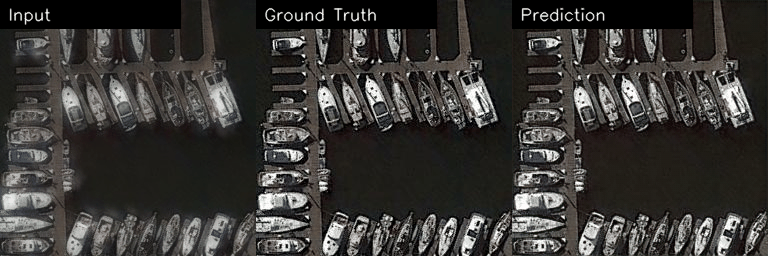
\includegraphics[width=\textwidth]{images/501.png}
        \\
        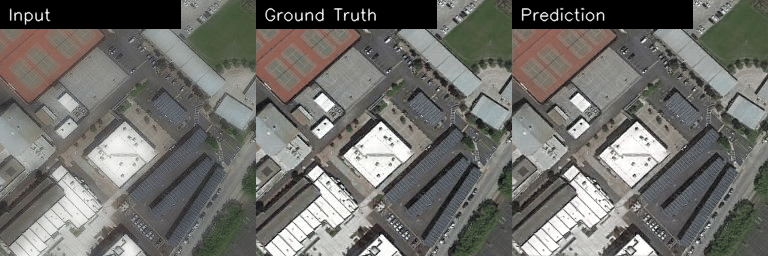
\includegraphics[width=\textwidth]{images/502.png}
        \\
        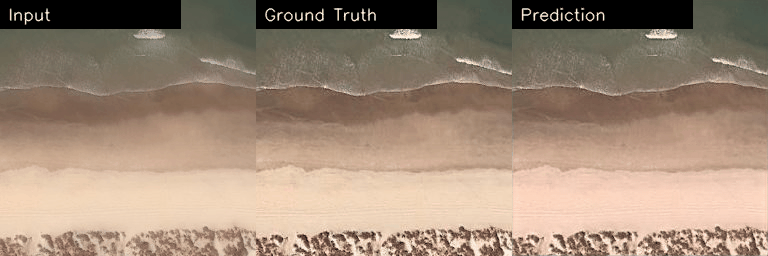
\includegraphics[width=\textwidth]{images/506.png}
        \caption{Turbulence strength 0.50.}
    \end{subfigure}
    \begin{subfigure}[b]{0.33\textwidth}
        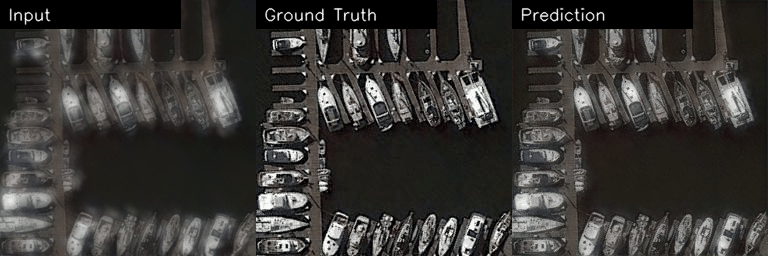
\includegraphics[width=\textwidth]{images/751.png}
        \\
        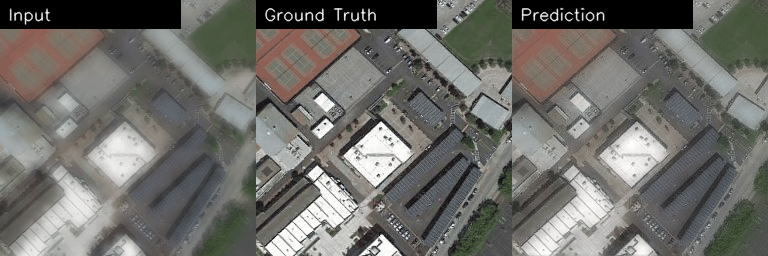
\includegraphics[width=\textwidth]{images/752.png}
        \\
        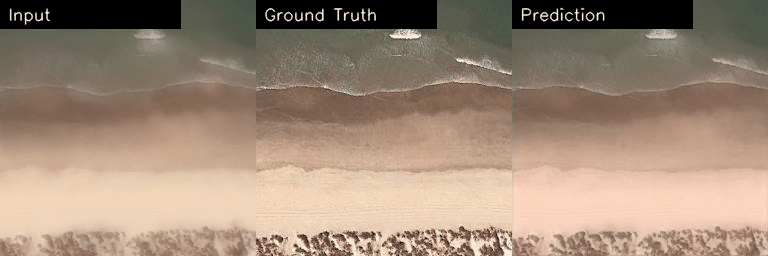
\includegraphics[width=\textwidth]{images/756.png}
        \caption{Turbulence strength 0.75.}
    \end{subfigure}
    \begin{subfigure}[b]{0.33\textwidth}
        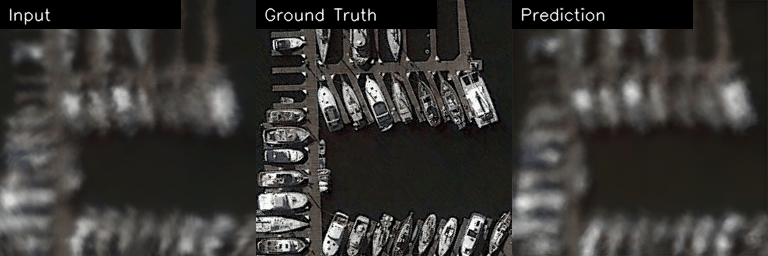
\includegraphics[width=\textwidth]{images/101.png}
        \\
        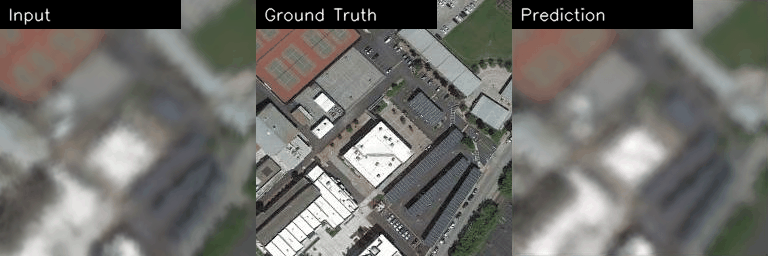
\includegraphics[width=\textwidth]{images/102.png}
        \\
        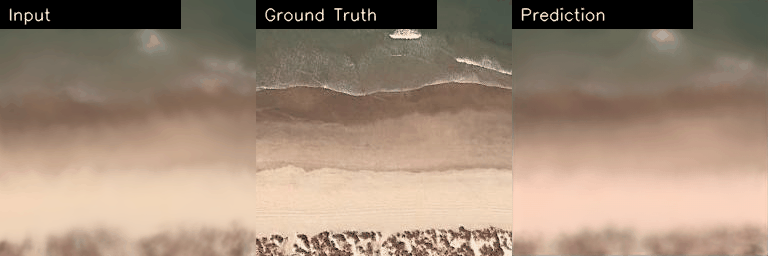
\includegraphics[width=\textwidth]{images/106.png}
        \caption{Turbulence strength 1.0.}
    \end{subfigure}
    \begin{subfigure}[b]{0.33\textwidth}
        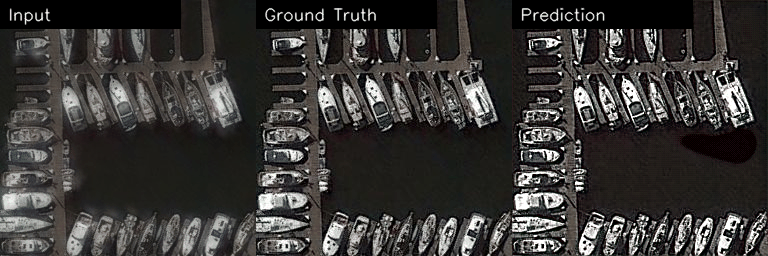
\includegraphics[width=\textwidth]{images/50175.png}
        \\
        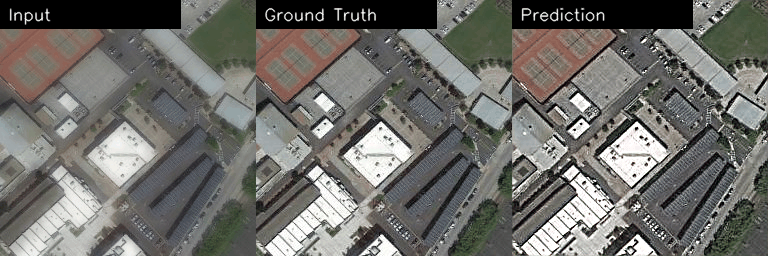
\includegraphics[width=\textwidth]{images/50275.png}
        \\
        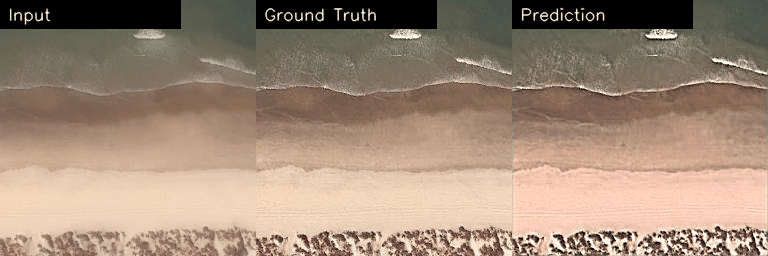
\includegraphics[width=\textwidth]{images/50675.png}
        \caption{Turbulence strength 0.50.}
    \end{subfigure}
    \begin{subfigure}[b]{0.33\textwidth}
        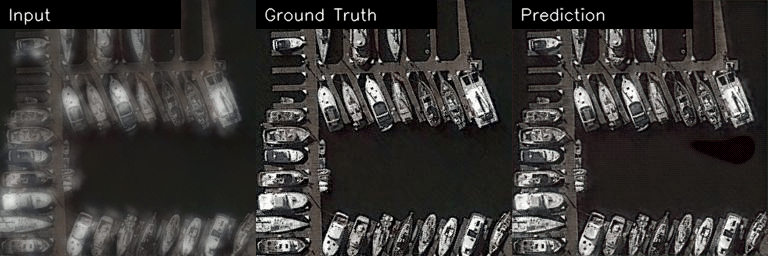
\includegraphics[width=\textwidth]{images/75175.png}
        \\
        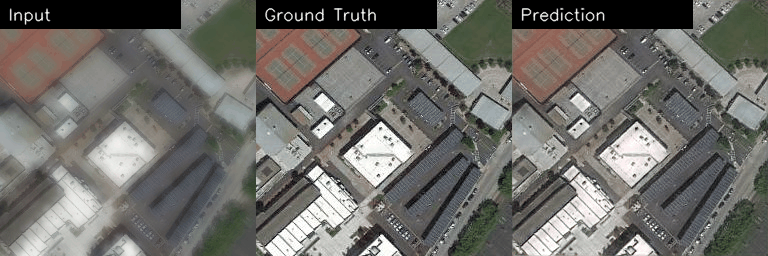
\includegraphics[width=\textwidth]{images/75275.png}
        \\
        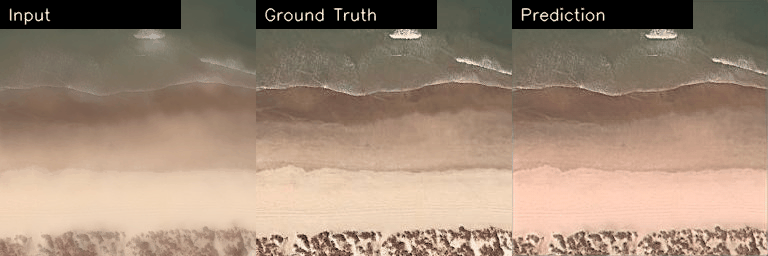
\includegraphics[width=\textwidth]{images/75675.png}
        \caption{Turbulence strength 0.75.}
    \end{subfigure}
    \begin{subfigure}[b]{0.33\textwidth}
        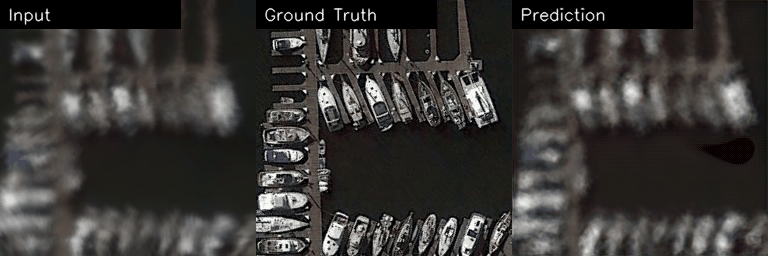
\includegraphics[width=\textwidth]{images/10175.png}
        \\
        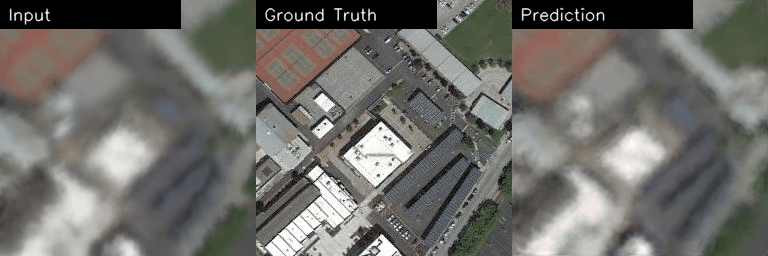
\includegraphics[width=\textwidth]{images/10275.png}
        \\
        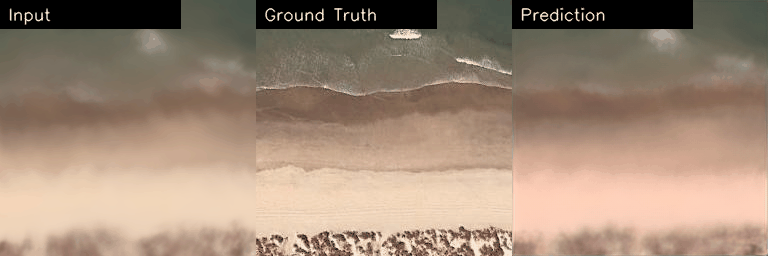
\includegraphics[width=\textwidth]{images/10675.png}
        \caption{Turbulence strength 1.0.}
    \end{subfigure}
    \begin{subfigure}[b]{0.33\textwidth}
        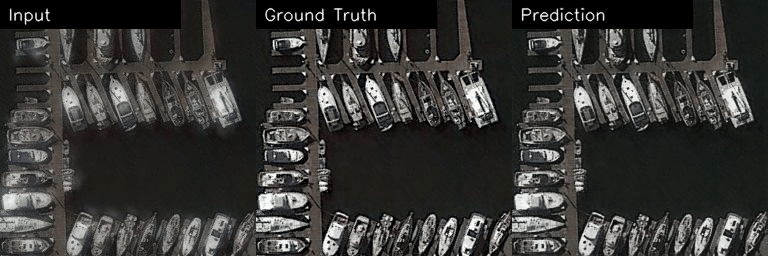
\includegraphics[width=\textwidth]{images/501gan.png}
        \\
        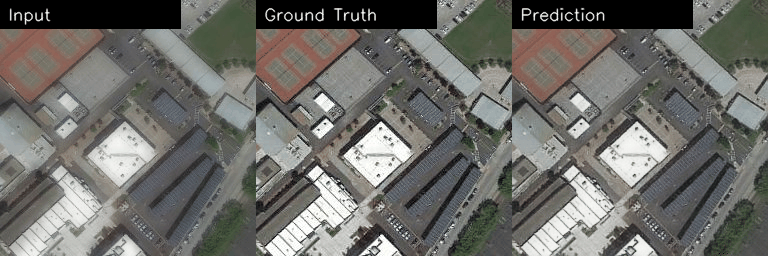
\includegraphics[width=\textwidth]{images/502gan.png}
        \\
        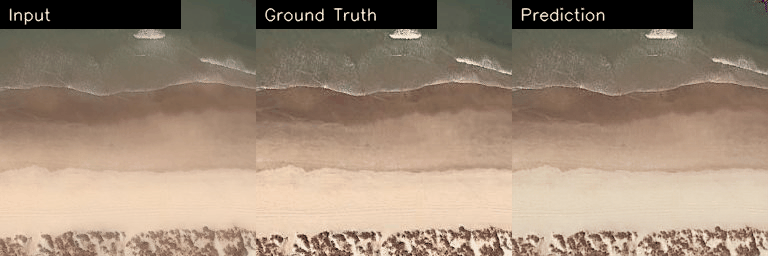
\includegraphics[width=\textwidth]{images/506gan.png}
        \caption{Turbulence strength 0.50.}
    \end{subfigure}
    \begin{subfigure}[b]{0.33\textwidth}
        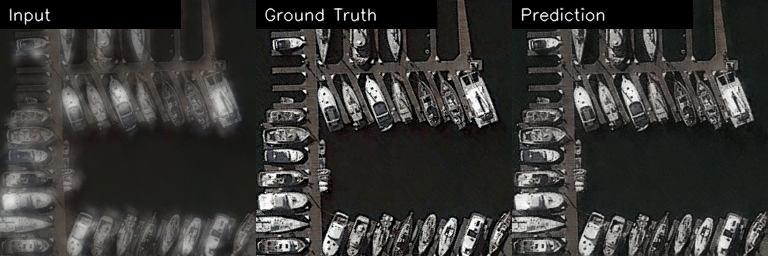
\includegraphics[width=\textwidth]{images/751gan.png}
        \\
        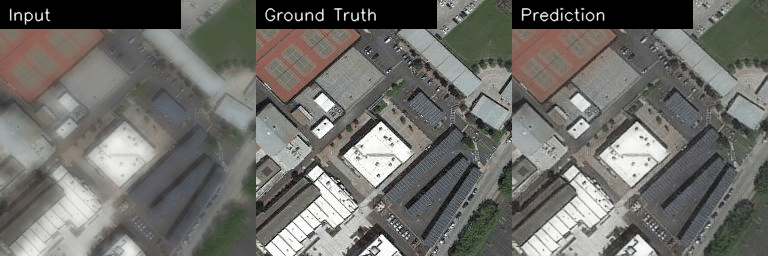
\includegraphics[width=\textwidth]{images/752gan.png}
        \\
        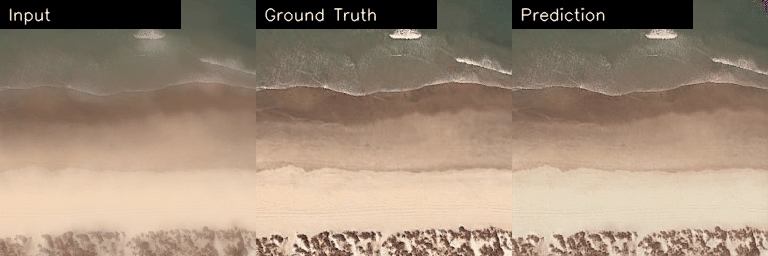
\includegraphics[width=\textwidth]{images/756gan.png}
        \caption{Turbulence strength 0.75.}
    \end{subfigure}
    \begin{subfigure}[b]{0.33\textwidth}
        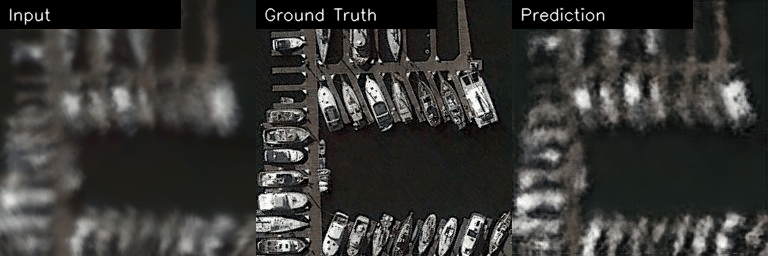
\includegraphics[width=\textwidth]{images/101gan.png}
        \\
        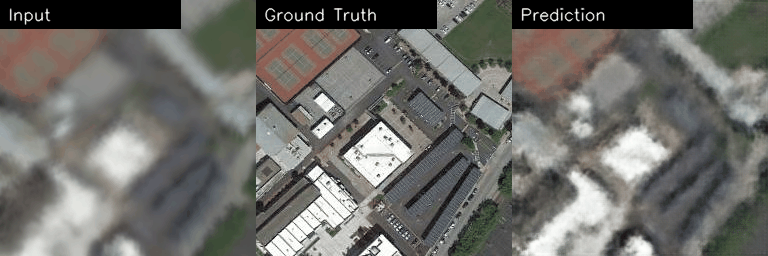
\includegraphics[width=\textwidth]{images/102gan.png}
        \\
        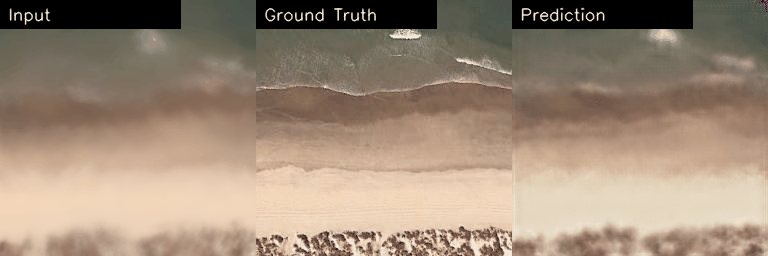
\includegraphics[width=\textwidth]{images/106gan.png}
        \caption{Turbulence strength 1.0.}
    \end{subfigure}
    \caption{Comparison of restoration results across different turbulence strengths (0.50, 0.75, 1.0) with 7-frame input. Figure (a), (b), (c) are the results of the 7-frame U-Net model trained on 0.50 turbulence strength, while Figure (d), (e), (f) are the results of the 7-frame U-Net model trained on 0.75 turbulence strength. Figure (g), (h), (i) are the results of TSR-WGAN trained on mixed 0.50 and 0.75 turbulence strengths.}
    \label{fig:compares}
\end{figure}
    \item For TSR-WGAN, seven-frame inference is much more stable than single-frame inference. At 0.50 and 0.75 turbulence strength, the seven-frame predictions retain smoother boundaries and fewer local distortions. At 1.0 strength, both settings become blurry, but the seven-frame output still preserves more coherent large-scale structure.
\end{itemize}
% \begin{figure}[H]
%     \centering
%     \begin{subfigure}[b]{0.33\textwidth}
%         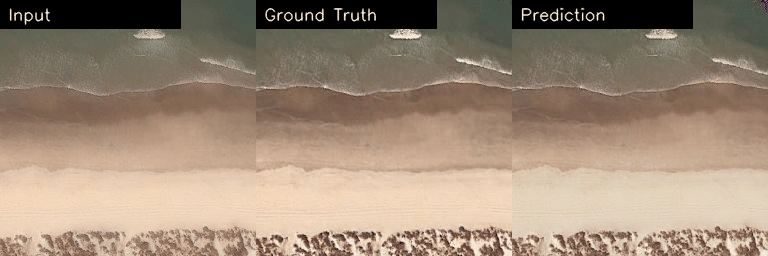
\includegraphics[width=\textwidth]{images/tsr_wgan_single_mild50_00006.png}
%         \caption{Single frame, 0.50.}
%     \end{subfigure}
%     \begin{subfigure}[b]{0.33\textwidth}
%         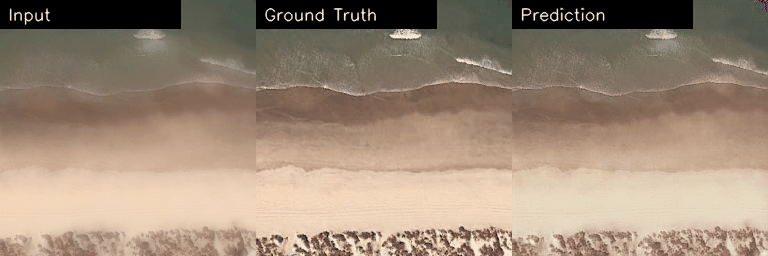
\includegraphics[width=\textwidth]{images/tsr_wgan_single_mild75_00006.png}
%         \caption{Single frame, 0.75.}
%     \end{subfigure}
%     \begin{subfigure}[b]{0.33\textwidth}
%         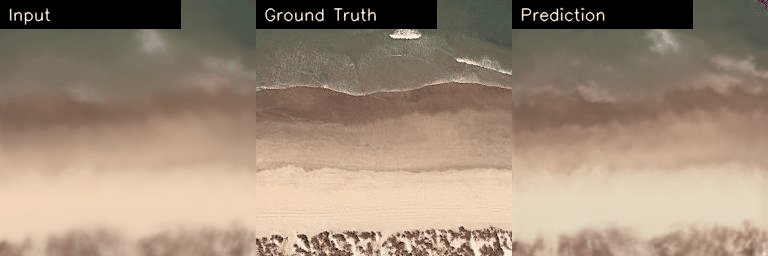
\includegraphics[width=\textwidth]{images/tsr_wgan_single_mild100_00006.png}
%         \caption{Single frame, 1.00.}
%     \end{subfigure}
%     \begin{subfigure}[b]{0.33\textwidth}
%         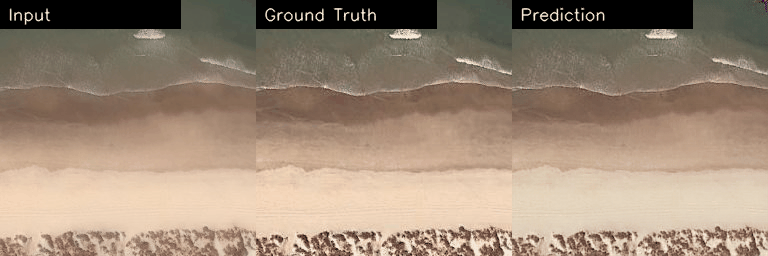
\includegraphics[width=\textwidth]{images/tsr_wgan_seven_mild50_00006.png}
%         \caption{Seven frames, 0.50.}
%     \end{subfigure}
%     \begin{subfigure}[b]{0.33\textwidth}
%         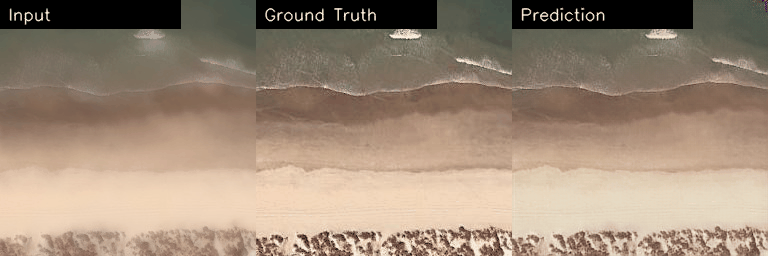
\includegraphics[width=\textwidth]{images/tsr_wgan_seven_mild75_00006.png}
%         \caption{Seven frames, 0.75.}
%     \end{subfigure}
%     \begin{subfigure}[b]{0.33\textwidth}
%         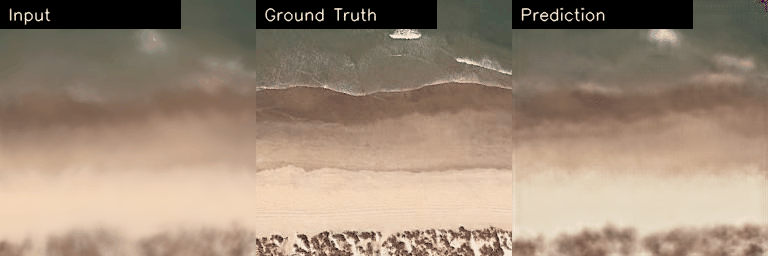
\includegraphics[width=\textwidth]{images/tsr_wgan_seven_mild100_00006.png}
%         \caption{Seven frames, 1.00.}
%     \end{subfigure}
%     \caption{TSR-WGAN qualitative generalization comparison across turbulence strengths and input settings. Each panel shows degraded input, clean target, and prediction.}
%     \label{fig:tsr_wgan_generalization_samples}
% \end{figure}


\subsection{Discussion}
The results point to several insights beyond the raw validation scores. First, temporal information is consistently useful across both architectures. Under the 0.50 training-time turbulence setting, the 7-frame U-Net reaches 35.341 dB PSNR and 0.9804 SSIM, compared with 31.483 dB and 0.9581 SSIM for the corresponding 1-frame model. Under the stronger 0.75 setting, the 7-frame model also outperforms the 1-frame model, with 31.783 dB and 0.9557 SSIM versus 29.463 dB and 0.9256 SSIM. TSR-WGAN shows the same trend even more strongly in the generalization sweep: at 0.75 test strength, seven-frame inference improves PSNR from 23.60 dB to 29.69 dB. The model benefits from multiple degraded observations because different frames preserve different local structures after random warping and blur.

Second, the U-Net experiments show that training turbulence strength behaves like a degradation-domain prior rather than a simple robustness knob. The model trained at 0.50 performs best when the test degradation is also mild, and its generalization curves decrease almost monotonically as turbulence strength increases. In contrast, the model trained at 0.75 does not peak at the easiest test setting. Its best performance appears around 0.70 test-time turbulence strength for both 1-frame and 7-frame inputs. This non-monotonic pattern suggests a mismatch effect: a model trained mainly to undo stronger blur and warping can over-correct or distort images from milder turbulence, while still struggling once the test corruption becomes more severe than the training distribution. The visual comparison at 0.50 test-time strength, where the 0.75-trained model tends to produce overly high contrast, is consistent with this explanation.

Third, TSR-WGAN occupies a different point in the tradeoff. Its validation score of 34.144 dB and 0.9712 SSIM is below the best in-distribution 0.50 U-Net, but it is trained on mixed 0.50 and 0.75 data and remains comparatively strong over a wider moderate-strength range. In particular, its seven-frame PSNR at 0.75 strength is 29.69 dB, above the 0.50-trained U-Net under the same test strength and close to the 0.75-trained U-Net. At 0.80 and 0.85, TSR-WGAN also keeps higher seven-frame PSNR and SSIM than the single-strength U-Net generalization baselines. This suggests that the temporal-spatial integration block and clip-based critic help the model exploit sequence redundancy under degradation mismatch.

Fourth, the adversarial objective does not automatically improve pixel metrics. TSR-WGAN includes WGAN-GP, VGG perceptual loss, and a large pixel-MSE term, so it is encouraged to produce realistic local structure while still staying close to the target. Even so, the direct $L_1$ U-Net objective remains best for mild in-distribution validation PSNR. Qualitatively, TSR-WGAN can preserve coherent large-scale boundaries, but its outputs sometimes appear darker or smoother than the ground truth. This is a common tension in restoration: adversarial and perceptual losses can improve visual plausibility, but PSNR and SSIM still reward conservative pixel alignment.

Finally, the experiments clarify the limits of the current system. A single U-Net trained at one turbulence strength does not provide uniform restoration quality across all turbulence levels. TSR-WGAN trained on mixed strengths improves moderate-range robustness, but it also degrades sharply near turbulence strength 1.0, where much of the fine-scale information is lost in every frame. These findings suggest that future models should train on broader or continuous turbulence-strength distributions, explicitly condition the network on degradation parameters such as estimated strength, wind, or blur severity, and test on real turbulence sequences to quantify the simulation-to-reality gap.

\section{Conclusion}
This project studies adaptive atmospheric turbulence restoration for remote sensing images through a compact but physically grounded learning pipeline. We combine clean remote sensing imagery from UC Merced and NWPU-RESISC45, a TurbulenceSim-style simulator for generating paired turbulence sequences, and two restoration families: a channel-stacked multi-frame U-Net and a sequence-aware TSR-WGAN. The best 0.50-strength 7-frame U-Net achieves 35.34 dB PSNR and 0.9804 SSIM on the validation split, while the stronger 0.75-strength U-Net setting still reaches 31.78 dB PSNR and 0.9557 SSIM. TSR-WGAN, trained on mixed 0.50 and 0.75 turbulence data, reaches 34.14 dB PSNR and 0.9712 SSIM on the validation split.

The main contribution of the project is a reproducible remote-sensing turbulence restoration pipeline that connects physically motivated synthetic degradation, sequence-based input aggregation, adversarial sequence restoration, and quantitative evaluation across turbulence strengths. The generalization experiments show that temporal information is valuable for both models, but also that degradation mismatch matters. The 0.50 U-Net performs very well in distribution but degrades under stronger corruption; the 0.75 U-Net is better tuned to moderate degradation but can over-restore milder inputs; and TSR-WGAN provides stronger mixed-strength robustness in the moderate range while still struggling under the most severe turbulence.

These findings point to several next steps. A stronger system should train on mixed or continuous turbulence strengths, condition the restoration network on degradation parameters, and extend the comparison to the diffusion models already scaffolded in the repository. Broader data coverage and real turbulence evaluation are also necessary to measure the simulation-to-reality gap. Overall, the current work provides a strong baseline and a clear empirical lesson: multi-frame evidence improves restoration, but robust adaptive optics restoration also requires explicit handling of turbulence-strength variation.

\begin{thebibliography}{9}

\bibitem[Arjovsky et~al.(2017)]{arjovsky2017wgan}
Martin Arjovsky, Soumith Chintala, and Leon Bottou.
Wasserstein generative adversarial networks.
In \emph{Proceedings of the International Conference on Machine Learning}, 2017.

\bibitem[Chimitt and Chan(2020)]{chimitt2020turbsim}
Nicholas Chimitt and Stanley H. Chan.
Simulating anisoplanatic turbulence by sampling inter-modal and spatially correlated Zernike coefficients.
\emph{arXiv preprint arXiv:2004.11210}, 2020.

\bibitem[Gulrajani et~al.(2017)]{gulrajani2017wgangp}
Ishaan Gulrajani, Faruk Ahmed, Martin Arjovsky, Vincent Dumoulin, and Aaron C. Courville.
Improved training of Wasserstein GANs.
In \emph{Advances in Neural Information Processing Systems}, 2017.

\bibitem[Hill et~al.(2024)]{hill2024review}
Paul Hill, Nantheera Anantrasirichai, Alin Achim, and David Bull.
Deep learning techniques for atmospheric turbulence removal: A review.
\emph{arXiv preprint arXiv:2409.14587}, 2024.

\bibitem[Jaiswal et~al.(2023)]{jaiswal2023physics}
Anshuman Jaiswal, Zhangyang Wang, and Stanley H. Chan.
Physics-driven turbulence image restoration with stochastic refinement.
In \emph{Proceedings of the IEEE/CVF International Conference on Computer Vision}, 2023.

\bibitem[Jin et~al.(2021)]{jin2021}
Kaixuan Jin, Yuhong Guo, Changshui Zhang, and Stanley H. Chan.
Neutralizing the impact of atmospheric turbulence on complex scene imaging via deep learning.
\emph{Nature Machine Intelligence}, 3(10):876--884, 2021.

\bibitem[Mei and Patel(2023)]{mei2023lttgan}
Kartikeya Mei and Vishal M. Patel.
LTT-GAN: Looking through turbulence by inverting GANs.
\emph{IEEE Journal of Selected Topics in Signal Processing}, 17(1):150--163, 2023.

\bibitem[Wang et~al.(2023)]{wang2023ddnm}
Yuan Wang, Haoyi Zhang, and Hongkai Xiong.
Zero-shot image restoration using denoising diffusion null-space model.
In \emph{International Conference on Learning Representations}, 2023.

\bibitem[Wang et~al.(2004)]{wang2004ssim}
Zhou Wang, Alan C. Bovik, Hamid R. Sheikh, and Eero P. Simoncelli.
Image quality assessment: from error visibility to structural similarity.
\emph{IEEE Transactions on Image Processing}, 13(4):600--612, 2004.

\end{thebibliography}

\end{document}